\documentclass[pra]{revtex4-1} 
 \usepackage{graphicx} 
\usepackage{color} 
\begin{document}
\section*{dephasing}
\begin{center}
\noindent Dependence of the thresholds on the features of the graph: 
  
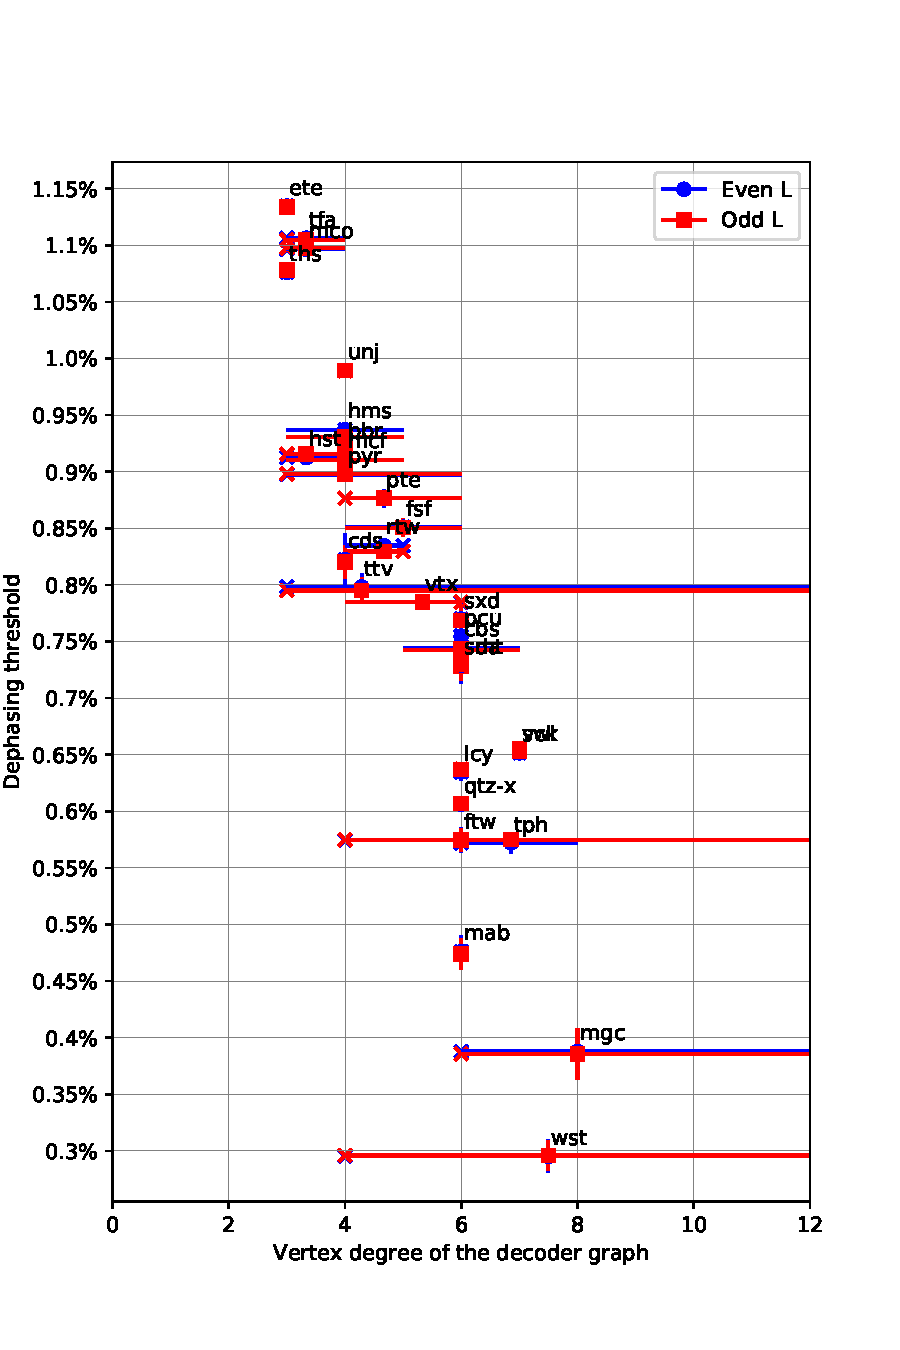
\includegraphics[width=.8\textwidth]{../graphs-paper2/thresholds-dephasing-decoder.pdf}

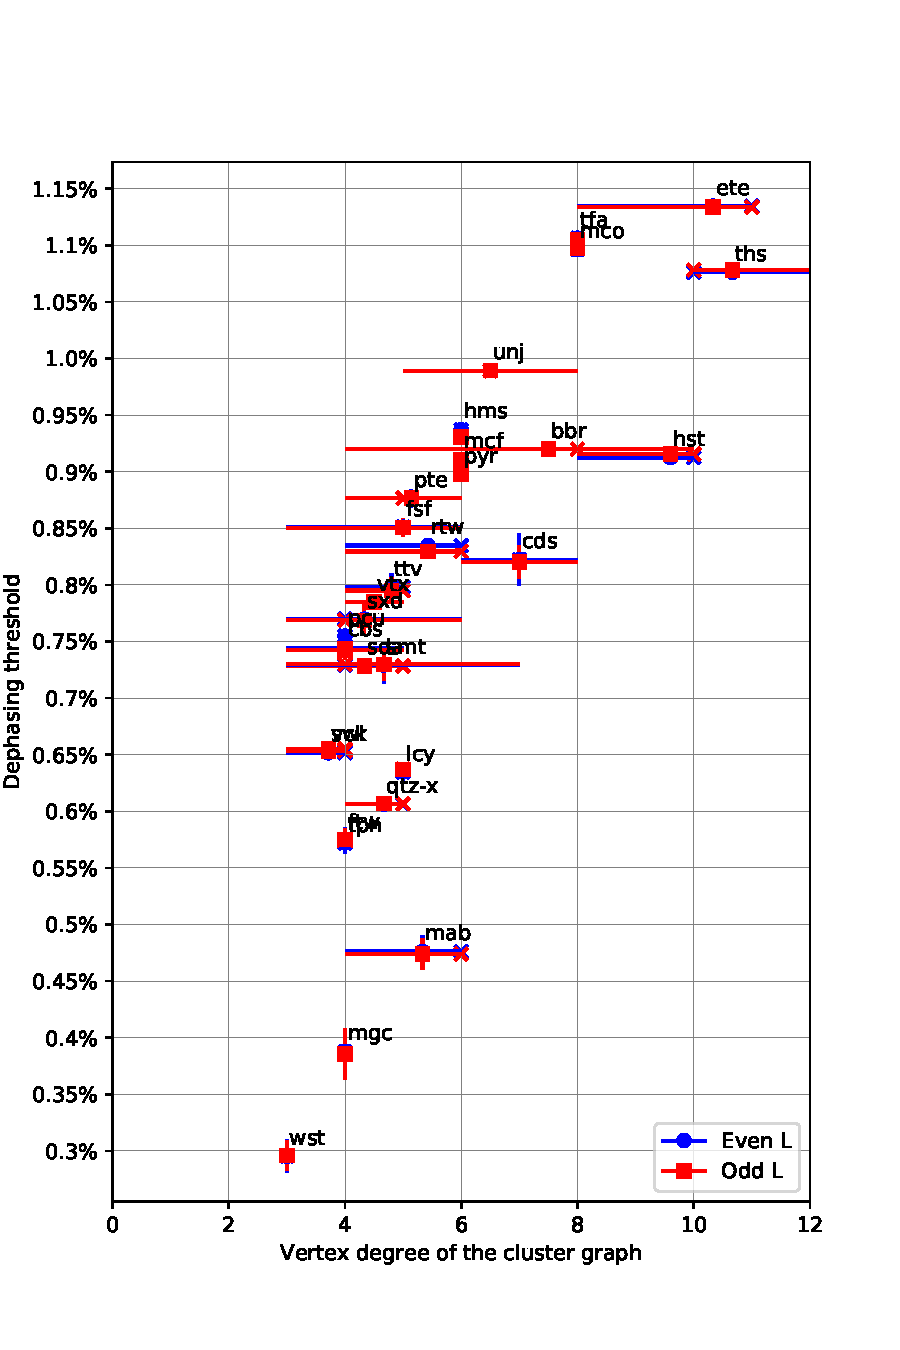
\includegraphics[width=.8\textwidth]{../graphs-paper2/thresholds-dephasing-cluster.pdf} \clearpage 

\clearpage
\subsection*{Ranking}
\begin{tabular}{|c|c|c|c|c|c|} \hline \bf Lattice & \bf Avg $d$ & \bf Avg $g$ & \bf Even Threshold & \bf Odd Threshold  & \bf Unified Threshold \\ \hline
\hline 
\color{blue}
ete &
\color{blue}
3.0 &
\color{blue}
10.33 &
\color{blue}
 $(1.135 \pm 0.002)\% $& 
\color{blue}
$(1.134 \pm 0.003)\% $ &
\color{blue}
$(1.134 \pm 0.002)\% $ \\
\color{blue}
tfa &
\color{blue}
3.33 &
\color{blue}
8.0 &
\color{blue}
 $(1.106 \pm 0.002)\% $& 
\color{blue}
$(1.105 \pm 0.002)\% $ &
\color{blue}
$(1.106 \pm 0.002)\% $ \\
\color{blue}
mco &
\color{blue}
3.33 &
\color{blue}
8.0 &
\color{blue}
 $(1.096 \pm 0.003)\% $& 
\color{blue}
$(1.098 \pm 0.003)\% $ &
\color{blue}
$(1.097 \pm 0.002)\% $ \\
\color{blue}
ths &
\color{blue}
3.0 &
\color{blue}
10.67 &
\color{blue}
 $(1.076 \pm 0.004)\% $& 
\color{blue}
$(1.078 \pm 0.004)\% $ &
\color{blue}
$(1.077 \pm 0.003)\% $ \\
\hline 
\color{blue}
unj &
\color{blue}
4.0 &
\color{blue}
6.5 &
\color{blue}
 $(0.989 \pm 0.005)\% $& 
\color{blue}
$(0.989 \pm 0.005)\% $ &
\color{blue}
$(0.989 \pm 0.003)\% $ \\
\color{blue}
hms &
\color{blue}
4.0 &
\color{blue}
6.0 &
\color{blue}
 $(0.937 \pm 0.004)\% $& 
\color{blue}
$(0.931 \pm 0.006)\% $ &
\color{blue}
$(0.951 \pm 0.027)\% $ \\
\color{blue}
bbr &
\color{blue}
4.0 &
\color{blue}
7.5 &
\color{blue}
 $(0.92 \pm 0.005)\% $& 
\color{blue}
$(0.92 \pm 0.005)\% $ &
\color{blue}
$(0.92 \pm 0.003)\% $ \\
\color{red}
hst &
\color{red}
3.33 &
\color{red}
9.6 &
\color{red}
 $(0.912 \pm 0.002)\% $& 
\color{red}
$(0.916 \pm 0.001)\% $ &
\color{red}
$(0.914 \pm 0.001)\% $ \\
\color{blue}
mcf &
\color{blue}
4.0 &
\color{blue}
6.0 &
\color{blue}
 $(0.911 \pm 0.004)\% $& 
\color{blue}
$(0.91 \pm 0.004)\% $ &
\color{blue}
$(0.91 \pm 0.003)\% $ \\
\color{blue}
pyr &
\color{blue}
4.0 &
\color{blue}
6.0 &
\color{blue}
 $(0.898 \pm 0.004)\% $& 
\color{blue}
$(0.898 \pm 0.004)\% $ &
\color{blue}
$(0.898 \pm 0.003)\% $ \\
\color{blue}
pte &
\color{blue}
4.67 &
\color{blue}
5.14 &
\color{blue}
 $(0.876 \pm 0.008)\% $& 
\color{blue}
$(0.877 \pm 0.006)\% $ &
\color{blue}
$(0.877 \pm 0.005)\% $ \\
\hline 
\color{blue}
fsf &
\color{blue}
5.0 &
\color{blue}
5.0 &
\color{blue}
 $(0.851 \pm 0.006)\% $& 
\color{blue}
$(0.851 \pm 0.008)\% $ &
\color{blue}
$(0.851 \pm 0.004)\% $ \\
\color{red}
rtw &
\color{red}
4.67 &
\color{red}
5.43 &
\color{red}
 $(0.835 \pm 0.003)\% $& 
\color{red}
$(0.829 \pm 0.003)\% $ &
\color{red}
$(0.833 \pm 0.002)\% $ \\
\hline 
\color{blue}
cds &
\color{blue}
4.0 &
\color{blue}
7.0 &
\color{blue}
 $(0.822 \pm 0.023)\% $& 
\color{blue}
$(0.82 \pm 0.015)\% $ &
\color{blue}
$(0.822 \pm 0.014)\% $ \\
\color{blue}
ttv &
\color{blue}
4.29 &
\color{blue}
4.8 &
\color{blue}
 $(0.798 \pm 0.012)\% $& 
\color{blue}
$(0.795 \pm 0.012)\% $ &
\color{blue}
$(0.797 \pm 0.008)\% $ \\
\hline 
\color{blue}
vtx &
\color{blue}
5.33 &
\color{blue}
4.5 &
\color{blue}
 $(0.785 \pm 0.005)\% $& 
\color{blue}
$(0.785 \pm 0.005)\% $ &
\color{blue}
$(0.785 \pm 0.003)\% $ \\
\color{blue}
sxd &
\color{blue}
6.0 &
\color{blue}
4.33 &
\color{blue}
 $(0.77 \pm 0.013)\% $& 
\color{blue}
$(0.769 \pm 0.014)\% $ &
\color{blue}
$(0.769 \pm 0.008)\% $ \\
\color{blue}
pcu &
\color{blue}
6.0 &
\color{blue}
4.0 &
\color{blue}
 $(0.755 \pm 0.007)\% $& 
\color{blue}
$(0.744 \pm 0.01)\% $ &
\color{blue}
$(0.759 \pm 0.013)\% $ \\
\color{blue}
cbs &
\color{blue}
6.0 &
\color{blue}
4.0 &
\color{blue}
 $(0.744 \pm 0.004)\% $& 
\color{blue}
$(0.742 \pm 0.004)\% $ &
\color{blue}
$(0.744 \pm 0.002)\% $ \\
\color{blue}
sda &
\color{blue}
6.0 &
\color{blue}
4.33 &
\color{blue}
 $(0.729 \pm 0.004)\% $& 
\color{blue}
$(0.728 \pm 0.004)\% $ &
\color{blue}
$(0.729 \pm 0.003)\% $ \\
\color{blue}
smt &
\color{blue}
6.0 &
\color{blue}
4.67 &
\color{blue}
 $(0.729 \pm 0.016)\% $& 
\color{blue}
$(0.73 \pm 0.014)\% $ &
\color{blue}
$(0.729 \pm 0.01)\% $ \\
\hline 
\color{blue}
swl &
\color{blue}
7.0 &
\color{blue}
3.71 &
\color{blue}
 $(0.652 \pm 0.003)\% $& 
\color{blue}
$(0.655 \pm 0.002)\% $ &
\color{blue}
$(0.653 \pm 0.002)\% $ \\
\color{blue}
vck &
\color{blue}
7.0 &
\color{blue}
3.71 &
\color{blue}
 $(0.653 \pm 0.003)\% $& 
\color{blue}
$(0.653 \pm 0.003)\% $ &
\color{blue}
$(0.653 \pm 0.002)\% $ \\
\hline 
\color{blue}
lcy &
\color{blue}
6.0 &
\color{blue}
5.0 &
\color{blue}
 $(0.635 \pm 0.007)\% $& 
\color{blue}
$(0.637 \pm 0.005)\% $ &
\color{blue}
$(0.636 \pm 0.004)\% $ \\
\color{blue}
qtz-x &
\color{blue}
6.0 &
\color{blue}
4.67 &
\color{blue}
 $(0.606 \pm 0.006)\% $& 
\color{blue}
$(0.607 \pm 0.005)\% $ &
\color{blue}
$(0.606 \pm 0.003)\% $ \\
\color{blue}
ftw &
\color{blue}
6.0 &
\color{blue}
4.0 &
\color{blue}
 $(0.574 \pm 0.011)\% $& 
\color{blue}
$(0.575 \pm 0.01)\% $ &
\color{blue}
$(0.575 \pm 0.007)\% $ \\
\color{blue}
tph &
\color{blue}
6.86 &
\color{blue}
4.0 &
\color{blue}
 $(0.572 \pm 0.009)\% $& 
\color{blue}
$(0.575 \pm 0.004)\% $ &
\color{blue}
$(0.574 \pm 0.004)\% $ \\
\color{blue}
mab &
\color{blue}
6.0 &
\color{blue}
5.33 &
\color{blue}
 $(0.476 \pm 0.014)\% $& 
\color{blue}
$(0.474 \pm 0.014)\% $ &
\color{blue}
$(0.476 \pm 0.009)\% $ \\
\hline 
\color{blue}
mgc &
\color{blue}
8.0 &
\color{blue}
4.0 &
\color{blue}
 $(0.388 \pm 0.018)\% $& 
\color{blue}
$(0.386 \pm 0.022)\% $ &
\color{blue}
$(0.387 \pm 0.013)\% $ \\
\color{blue}
wst &
\color{blue}
7.5 &
\color{blue}
3.0 &
\color{blue}
 $(0.295 \pm 0.015)\% $& 
\color{blue}
$(0.296 \pm 0.013)\% $ &
\color{blue}
$(0.296 \pm 0.009)\% $ \\
\hline \end{tabular}
\clearpage
\noindent Precision in terms of compute time: 
  
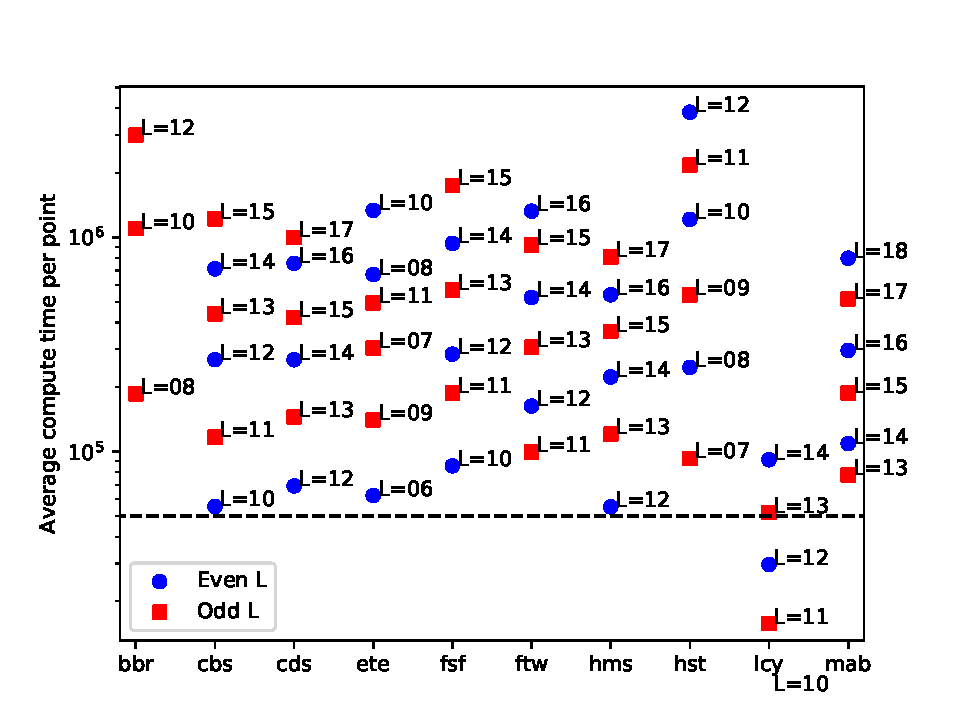
\includegraphics[width=.8\textwidth]{../graphs-paper2/time-dephasing-0.pdf}

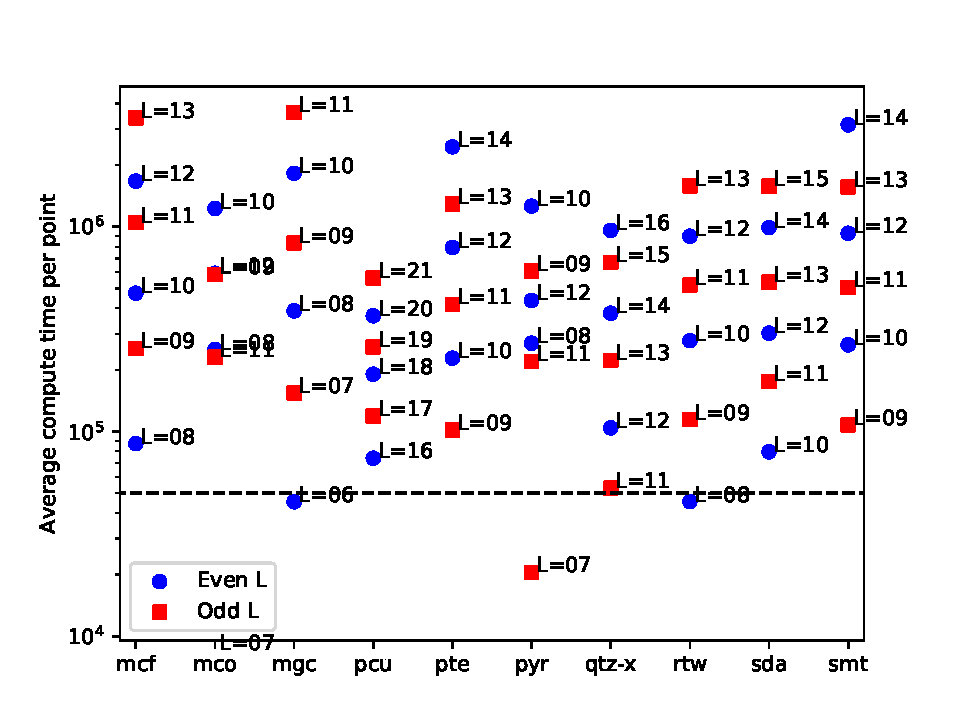
\includegraphics[width=.8\textwidth]{../graphs-paper2/time-dephasing-1.pdf}

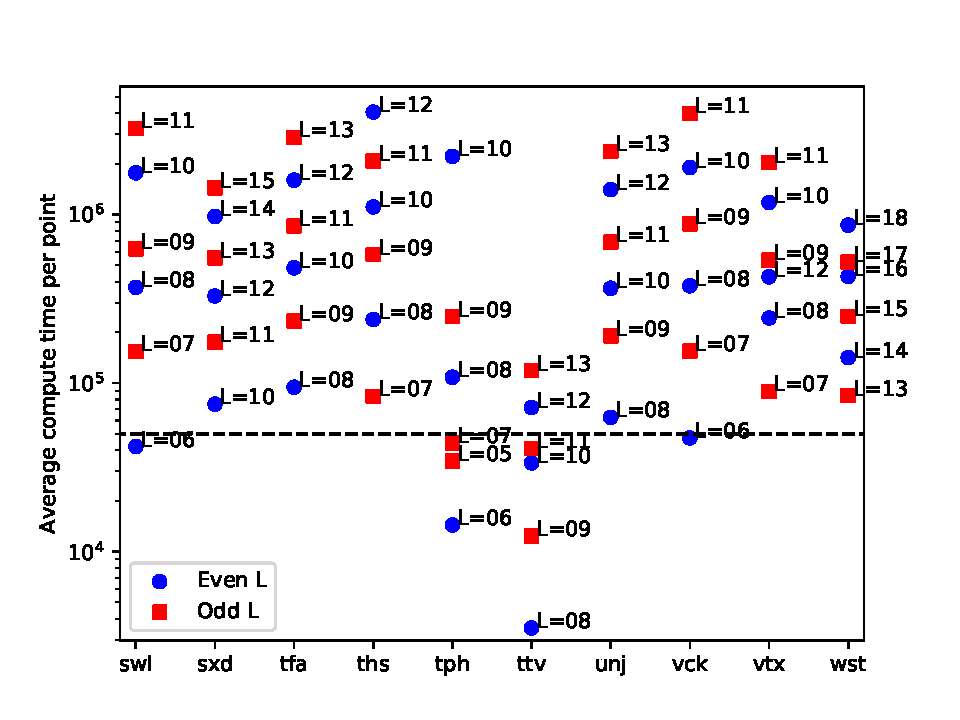
\includegraphics[width=.8\textwidth]{../graphs-paper2/time-dephasing-2.pdf}

\end{center} 

\clearpage 

\subsection*{bbr}
\noindent Increase of the failure rate with error probability: 
  
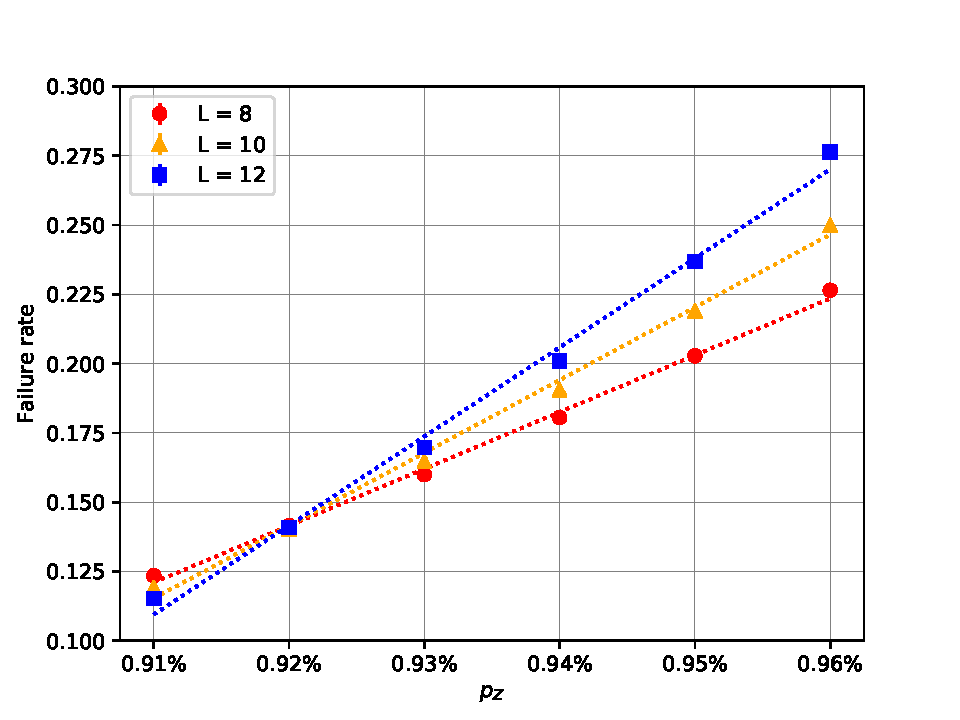
\includegraphics[width=.49\textwidth]{../graphs-paper2/bbr-dephasing-even.pdf}
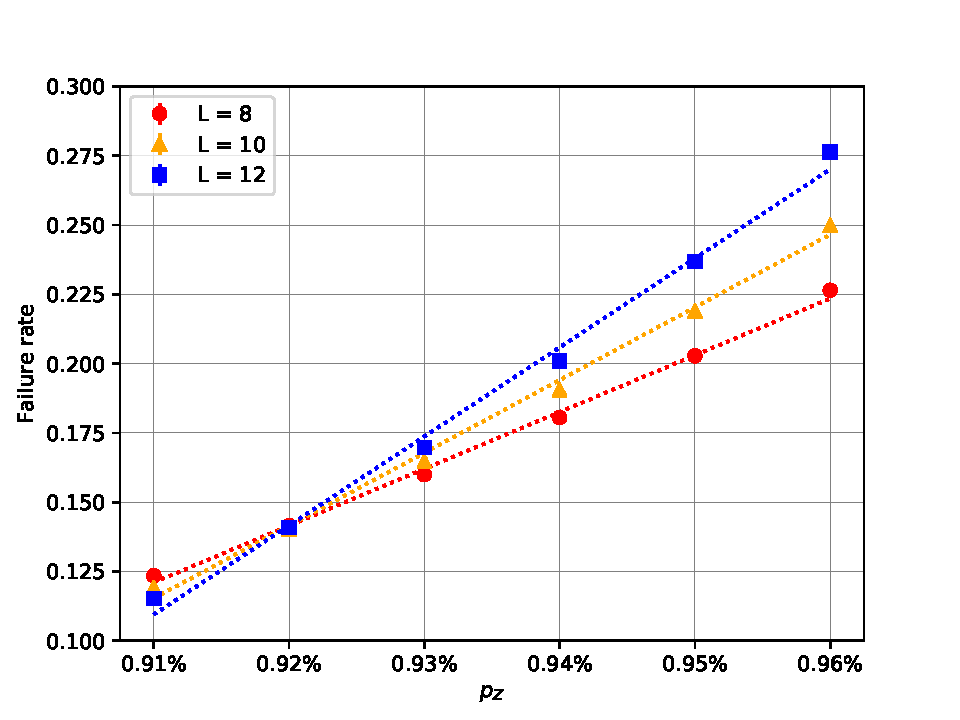
\includegraphics[width=.49\textwidth]{../graphs-paper2/bbr-dephasing-odd.pdf}

\noindent Fitting all points to a linear function $f(x) = A + Bx$, where $x=(p-p_{th})L^{\nu}$ for some $p_{th}$ and $\nu$: 
  
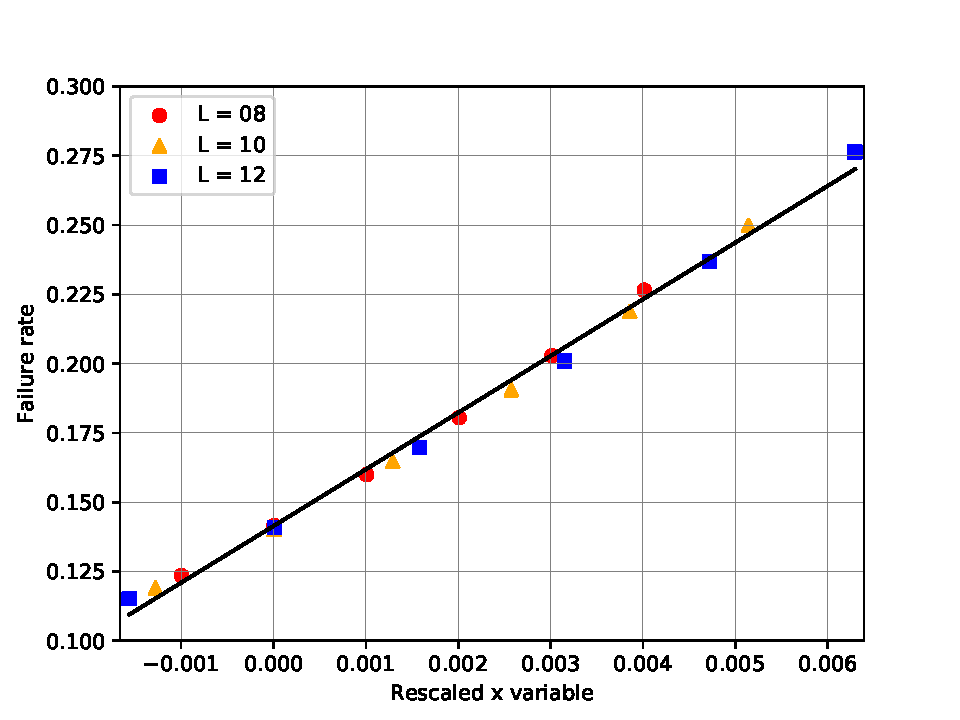
\includegraphics[width=.49\textwidth]{../graphs-paper2/bbr-dephasing-even-rescaled.pdf}
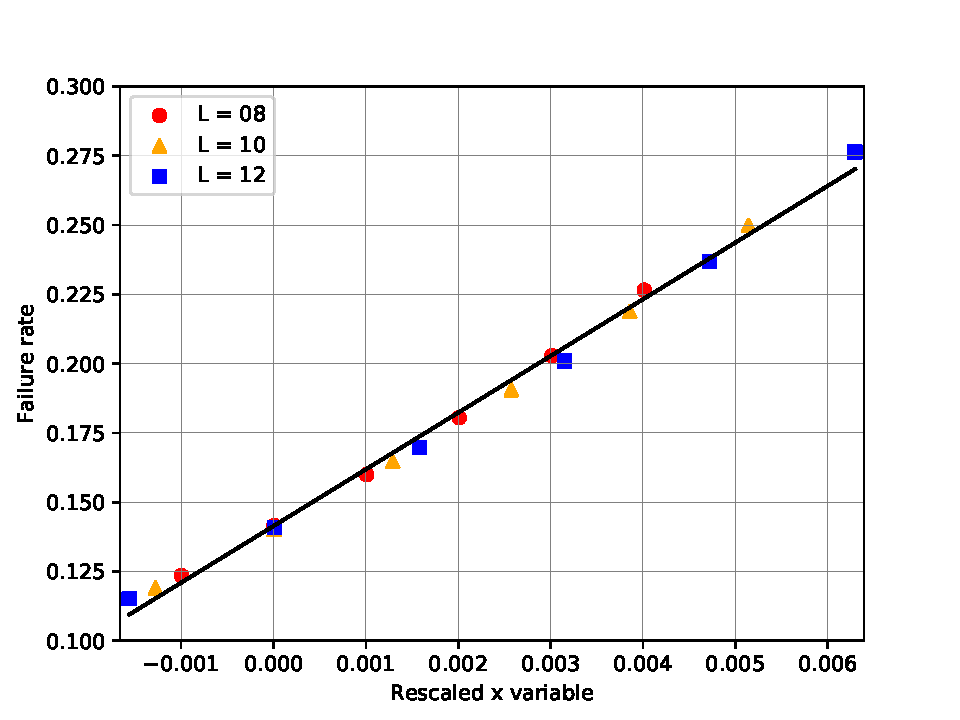
\includegraphics[width=.49\textwidth]{../graphs-paper2/bbr-dephasing-odd-rescaled.pdf}

\[  p_{even} = (0.92 \pm 0.005)\% \]
\[  p_{odd} = (0.92 \pm 0.005)\% \]
\clearpage 

Unified fit: \begin{center} 

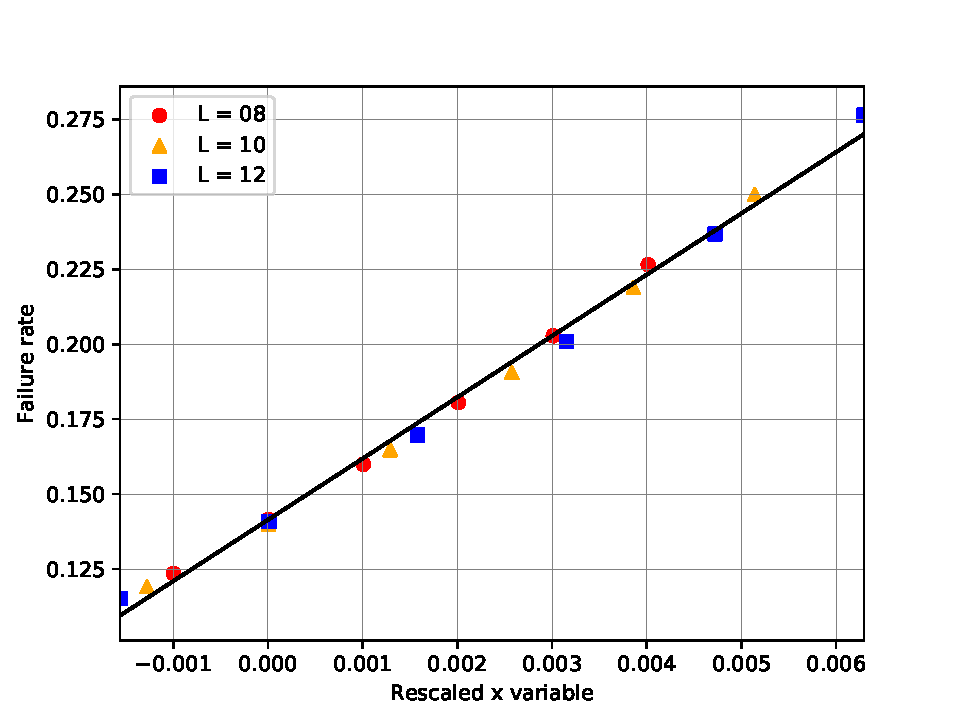
\includegraphics[width=.9\textwidth]{../graphs-paper2/bbr-dephasing-rescaled.pdf}
\[  p_{th} = (0.92 \pm 0.003)\% \] \end{center}
\clearpage 

\subsection*{cbs}
\noindent Increase of the failure rate with error probability: 
  
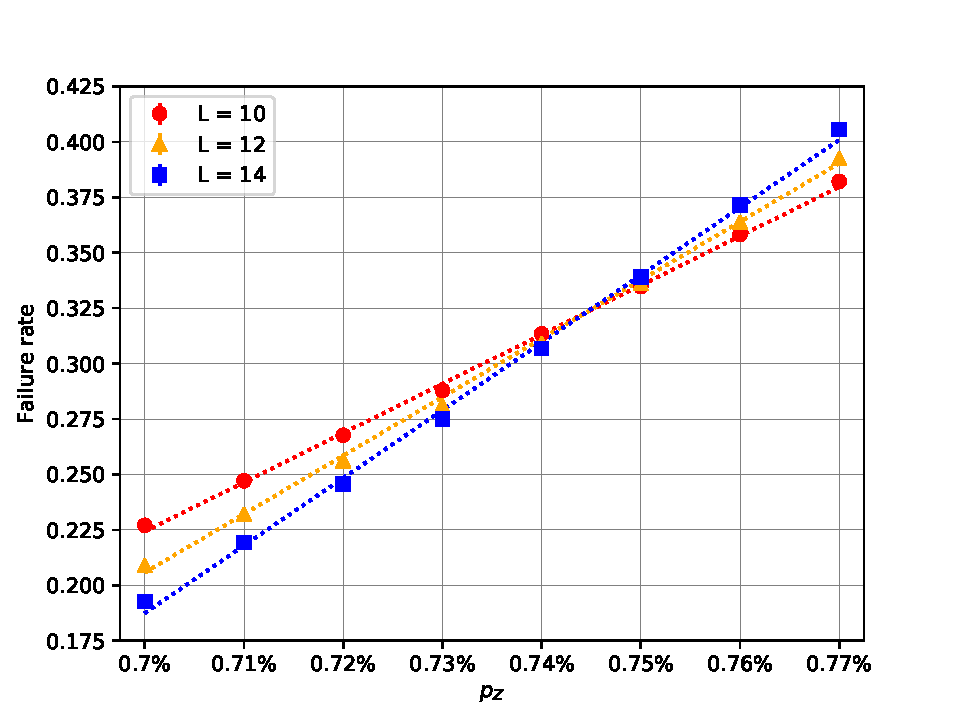
\includegraphics[width=.49\textwidth]{../graphs-paper2/cbs-dephasing-even.pdf}
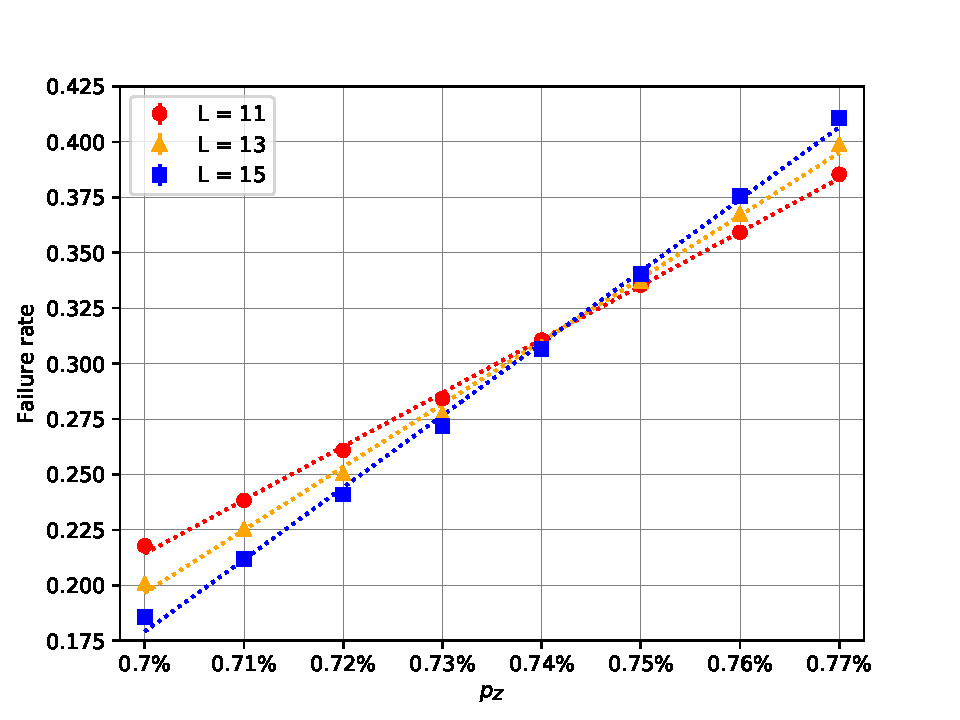
\includegraphics[width=.49\textwidth]{../graphs-paper2/cbs-dephasing-odd.pdf}

\noindent Fitting all points to a linear function $f(x) = A + Bx$, where $x=(p-p_{th})L^{\nu}$ for some $p_{th}$ and $\nu$: 
  
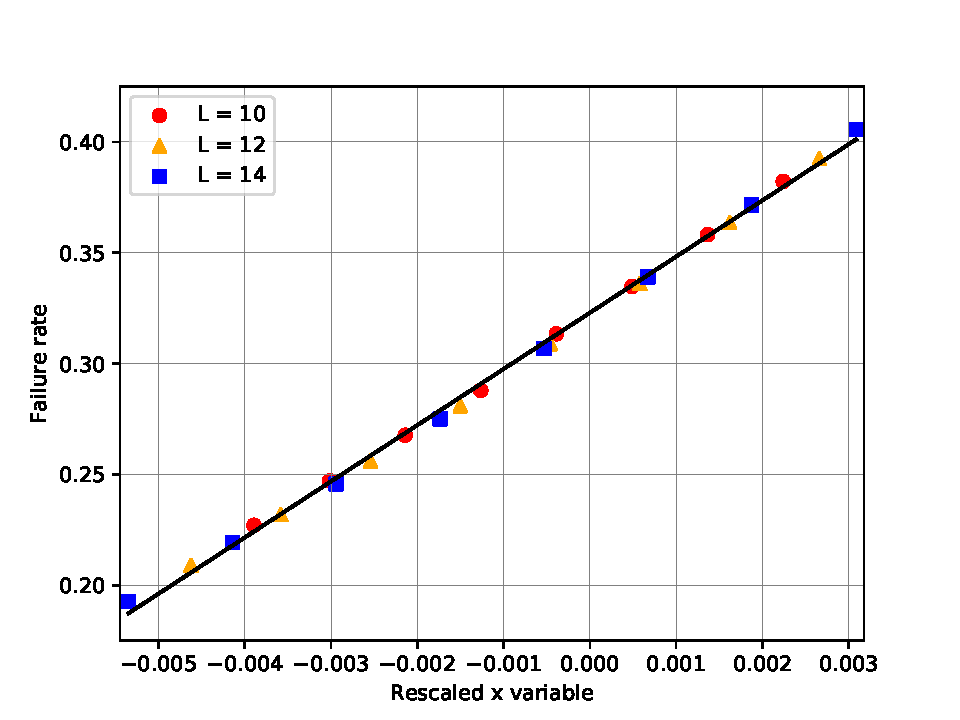
\includegraphics[width=.49\textwidth]{../graphs-paper2/cbs-dephasing-even-rescaled.pdf}
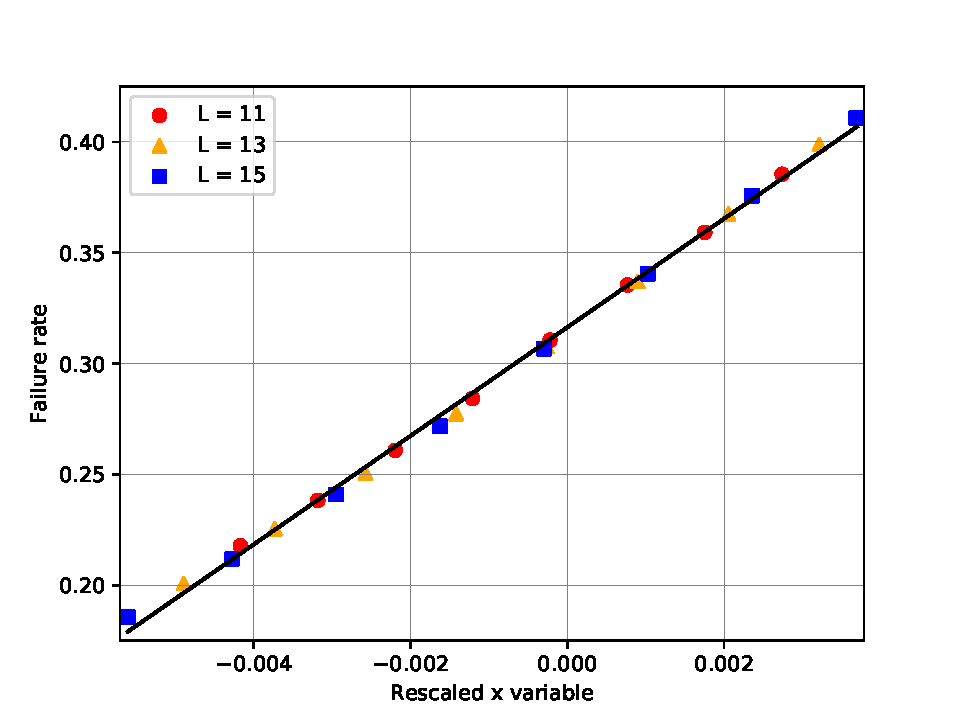
\includegraphics[width=.49\textwidth]{../graphs-paper2/cbs-dephasing-odd-rescaled.pdf}

\[  p_{even} = (0.744 \pm 0.004)\% \]
\[  p_{odd} = (0.742 \pm 0.004)\% \]
\clearpage 

Unified fit: \begin{center} 

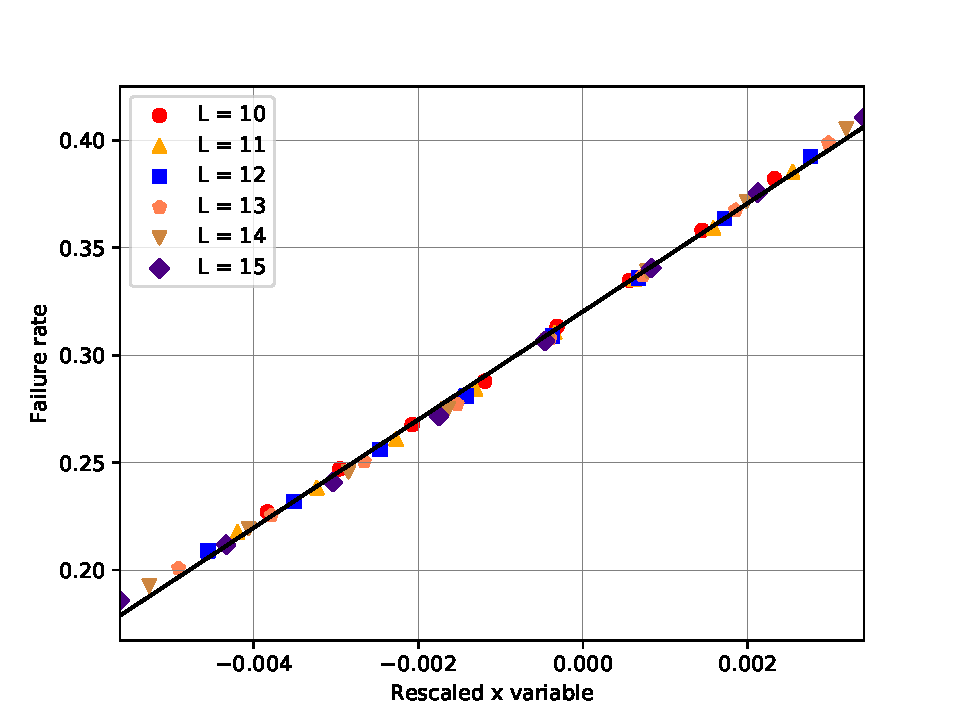
\includegraphics[width=.9\textwidth]{../graphs-paper2/cbs-dephasing-rescaled.pdf}
\[  p_{th} = (0.744 \pm 0.002)\% \] \end{center}
\clearpage 

\subsection*{cds}
\noindent Increase of the failure rate with error probability: 
  
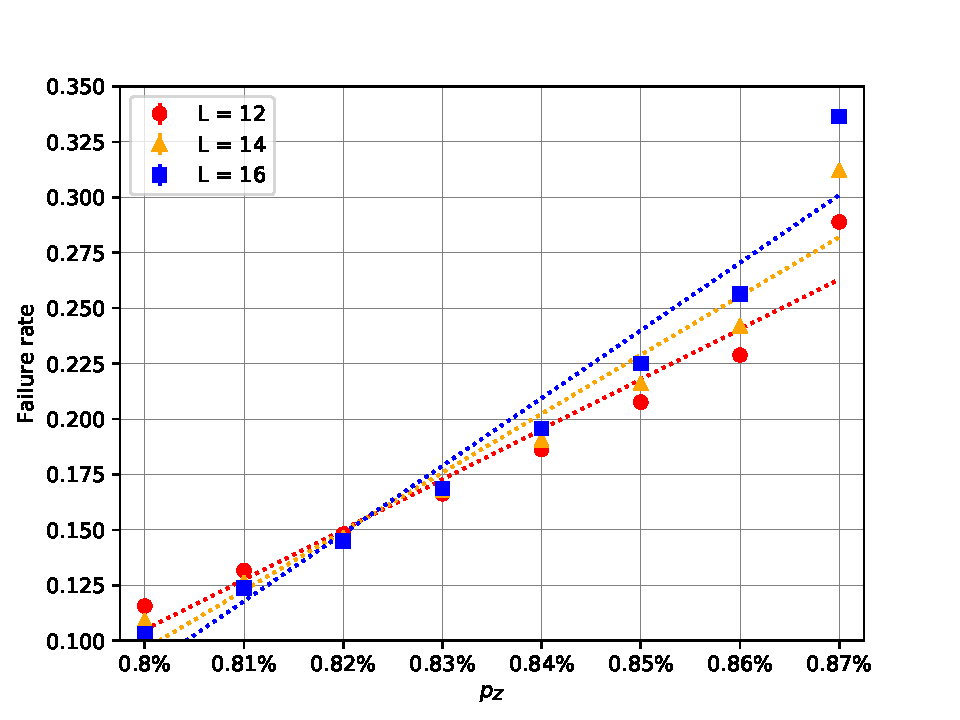
\includegraphics[width=.49\textwidth]{../graphs-paper2/cds-dephasing-even.pdf}
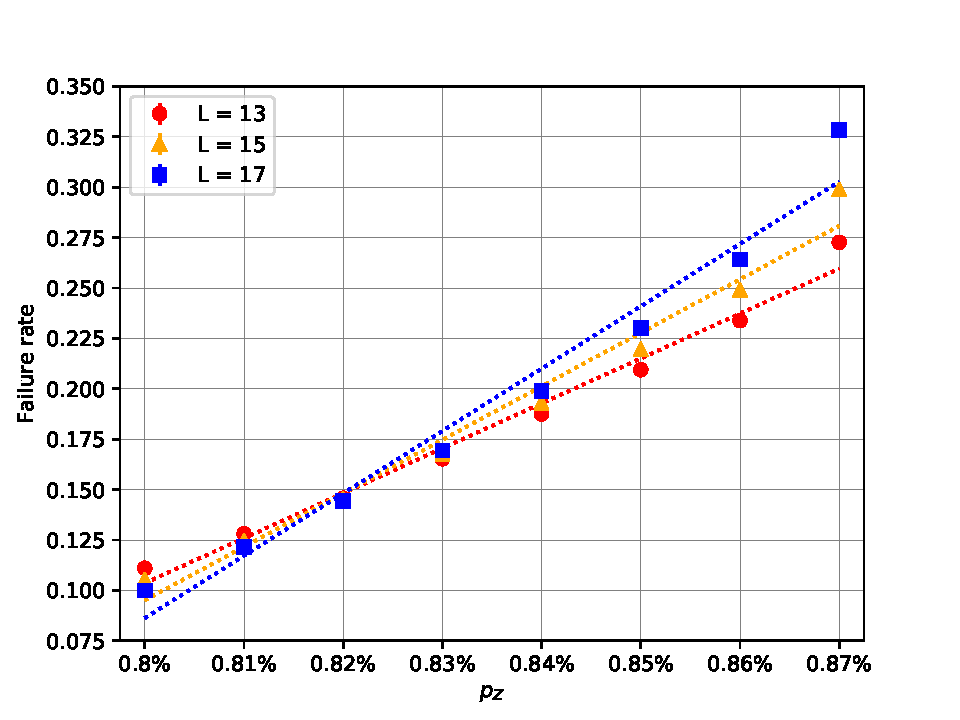
\includegraphics[width=.49\textwidth]{../graphs-paper2/cds-dephasing-odd.pdf}

\noindent Fitting all points to a linear function $f(x) = A + Bx$, where $x=(p-p_{th})L^{\nu}$ for some $p_{th}$ and $\nu$: 
  
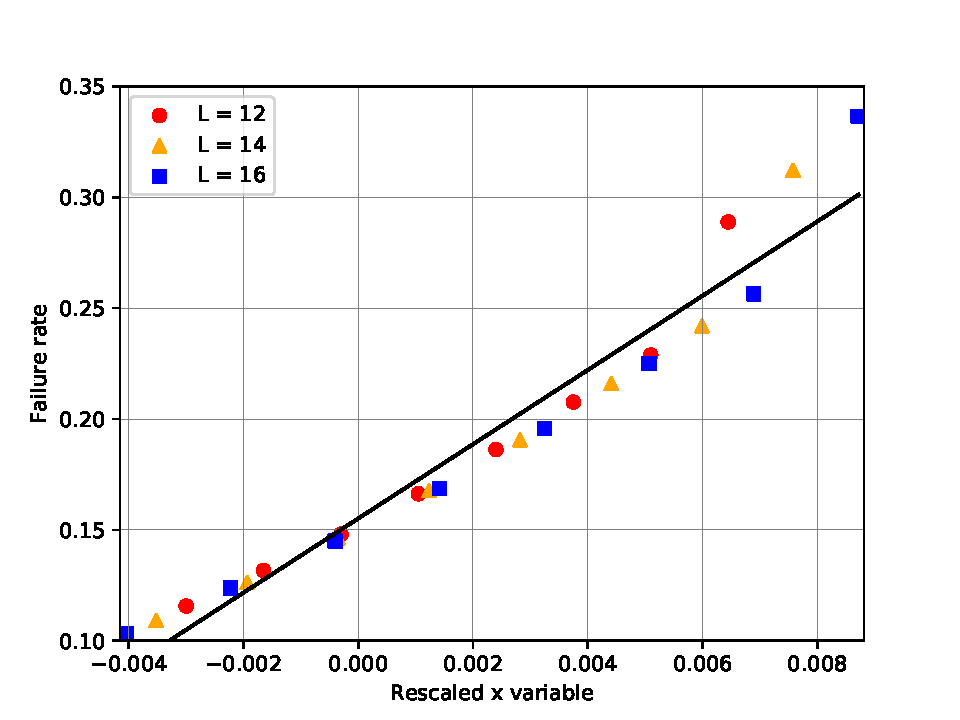
\includegraphics[width=.49\textwidth]{../graphs-paper2/cds-dephasing-even-rescaled.pdf}
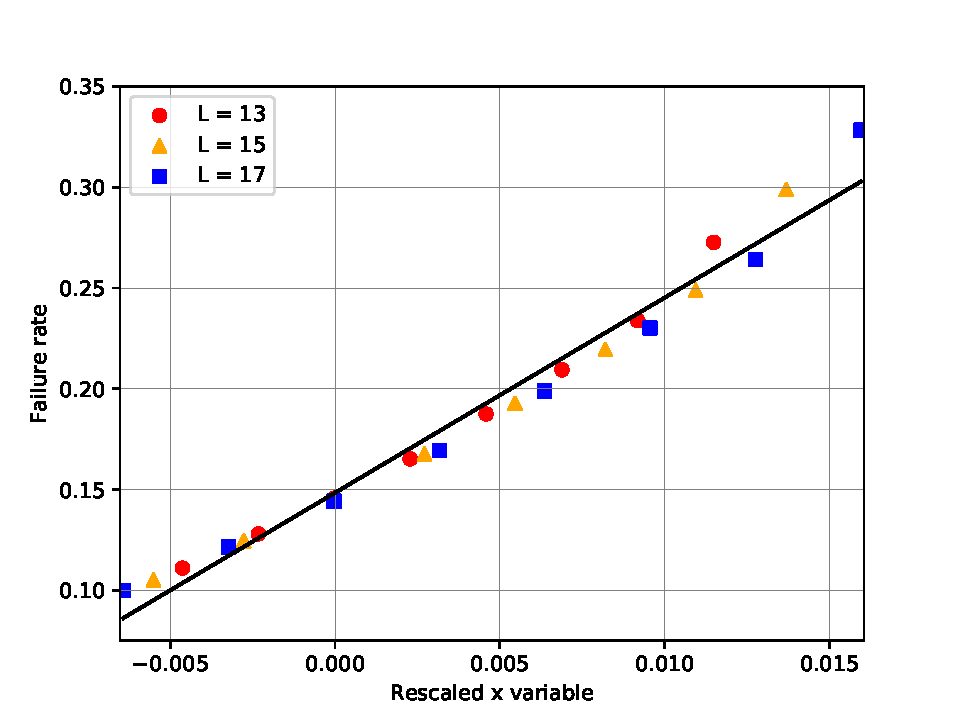
\includegraphics[width=.49\textwidth]{../graphs-paper2/cds-dephasing-odd-rescaled.pdf}

\[  p_{even} = (0.822 \pm 0.023)\% \]
\[  p_{odd} = (0.82 \pm 0.015)\% \]
\clearpage 

Unified fit: \begin{center} 

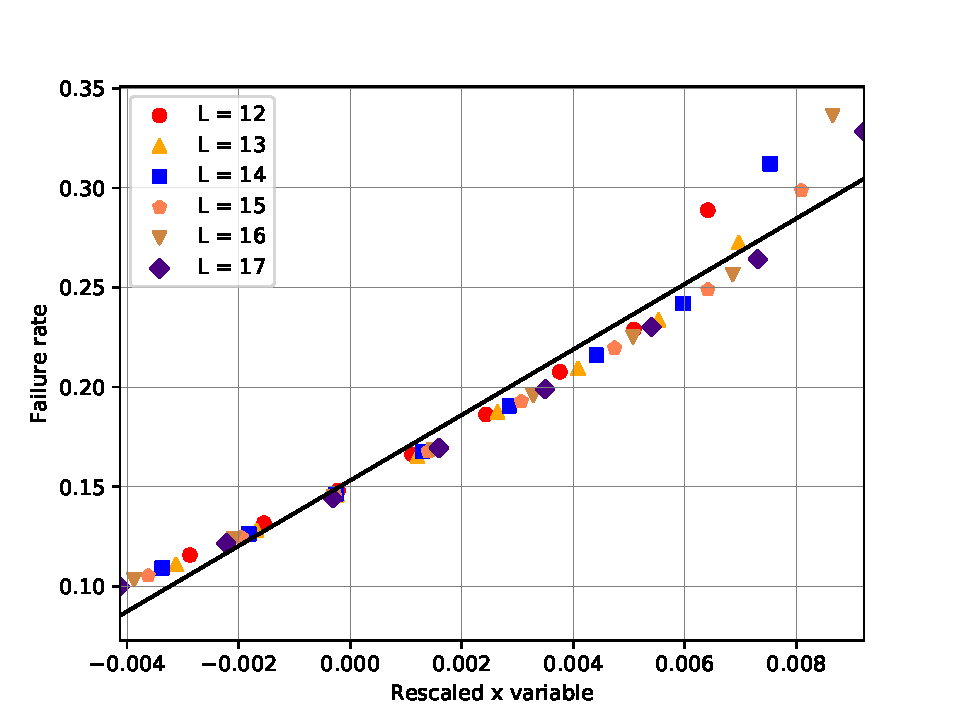
\includegraphics[width=.9\textwidth]{../graphs-paper2/cds-dephasing-rescaled.pdf}
\[  p_{th} = (0.822 \pm 0.014)\% \] \end{center}
\clearpage 

\subsection*{ete}
\noindent Increase of the failure rate with error probability: 
  
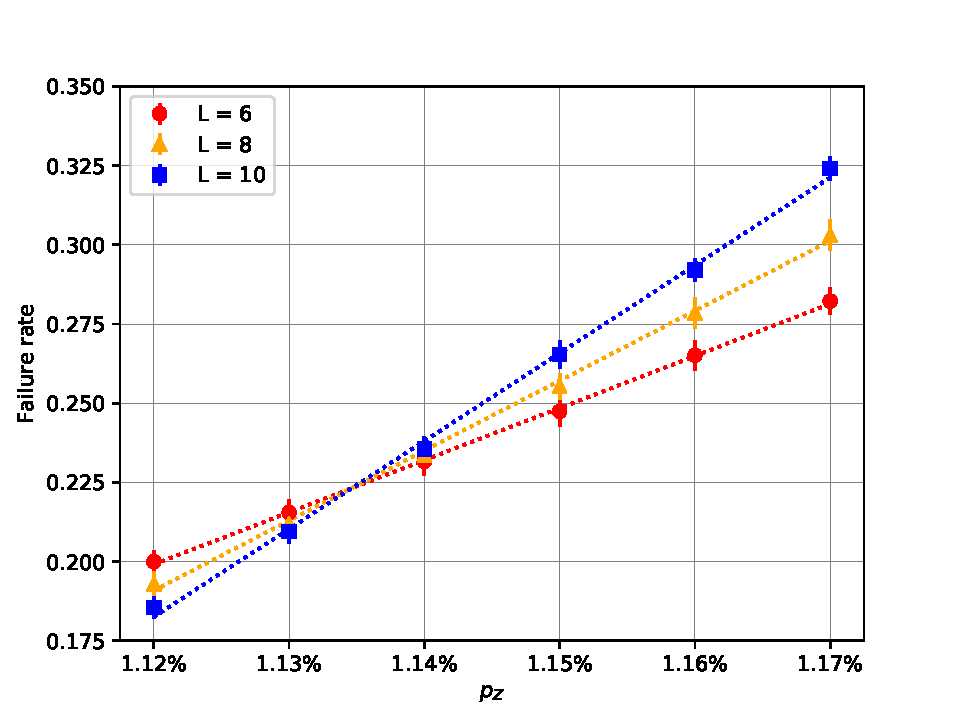
\includegraphics[width=.49\textwidth]{../graphs-paper2/ete-dephasing-even.pdf}
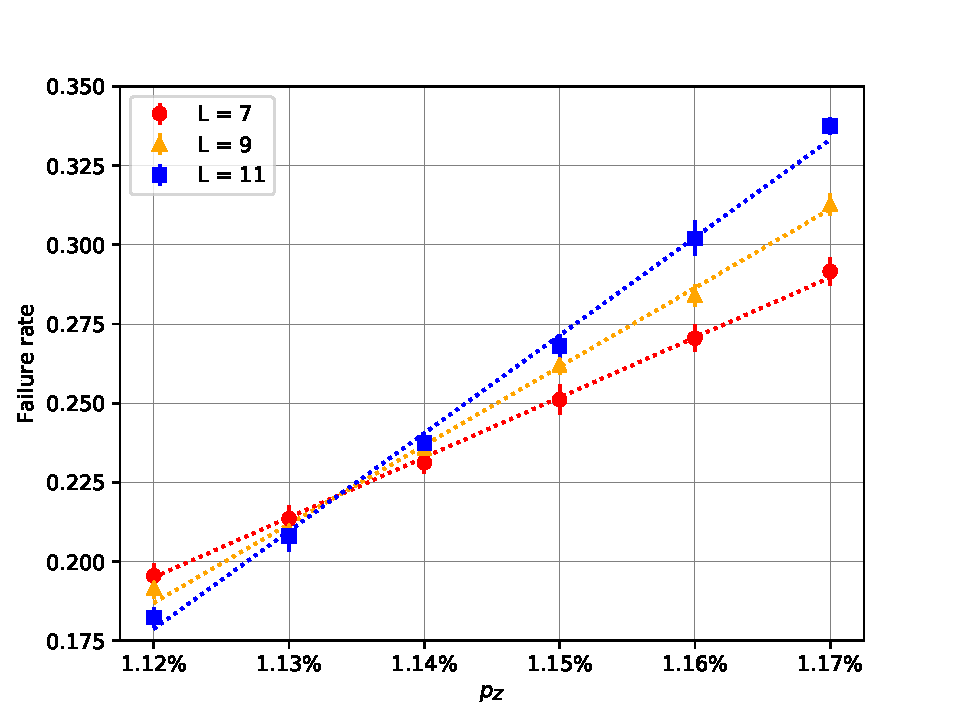
\includegraphics[width=.49\textwidth]{../graphs-paper2/ete-dephasing-odd.pdf}

\noindent Fitting all points to a linear function $f(x) = A + Bx$, where $x=(p-p_{th})L^{\nu}$ for some $p_{th}$ and $\nu$: 
  
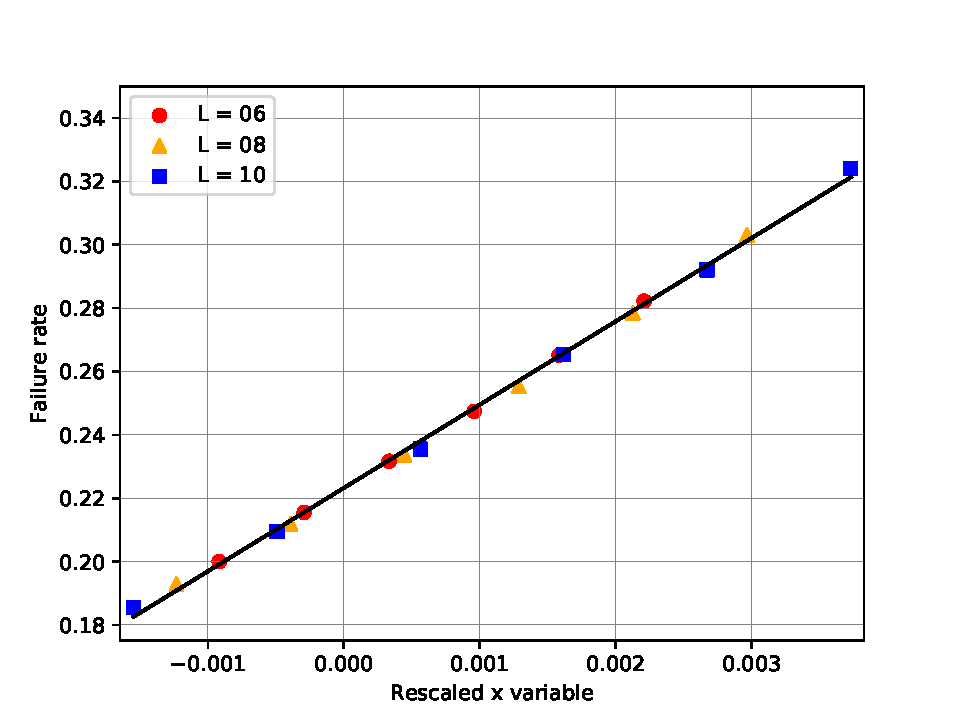
\includegraphics[width=.49\textwidth]{../graphs-paper2/ete-dephasing-even-rescaled.pdf}
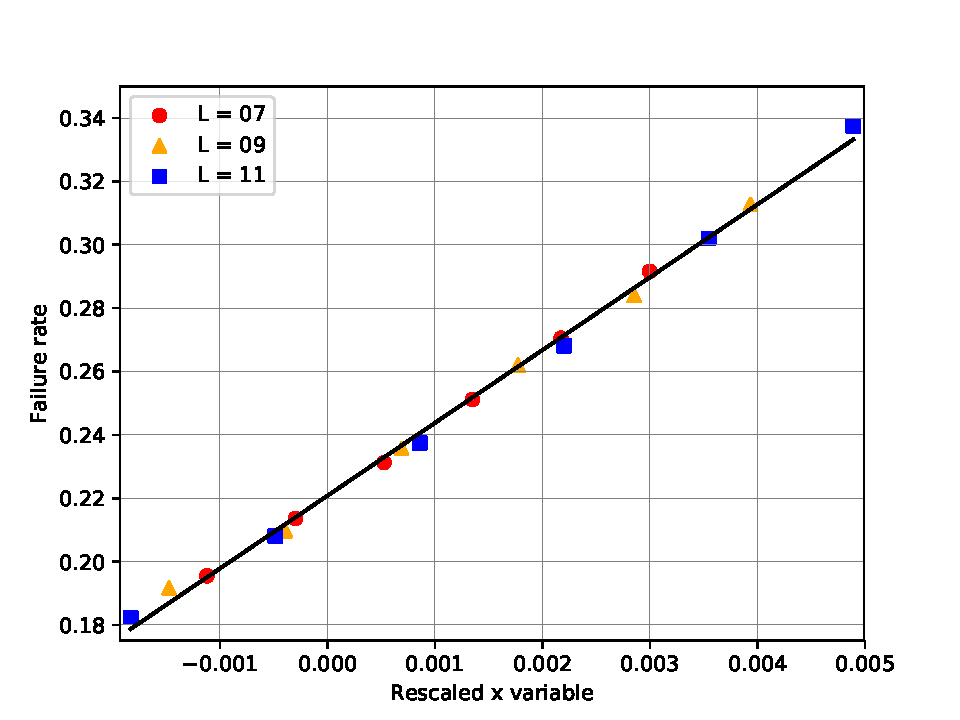
\includegraphics[width=.49\textwidth]{../graphs-paper2/ete-dephasing-odd-rescaled.pdf}

\[  p_{even} = (1.135 \pm 0.002)\% \]
\[  p_{odd} = (1.134 \pm 0.003)\% \]
\clearpage 

Unified fit: \begin{center} 

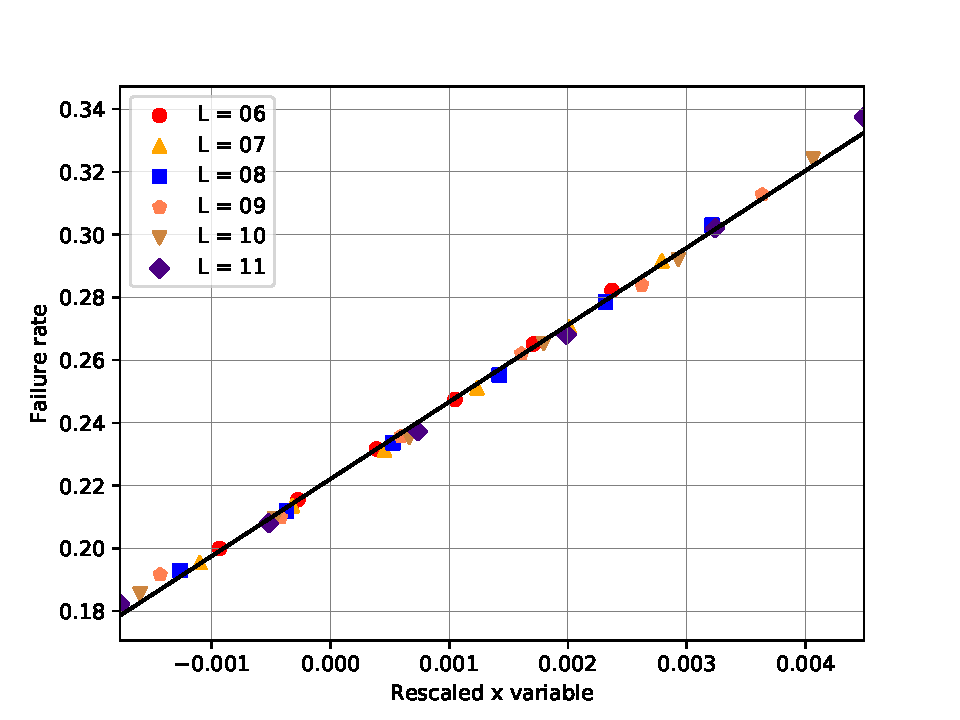
\includegraphics[width=.9\textwidth]{../graphs-paper2/ete-dephasing-rescaled.pdf}
\[  p_{th} = (1.134 \pm 0.002)\% \] \end{center}
\clearpage 

\subsection*{fsf}
\noindent Increase of the failure rate with error probability: 
  
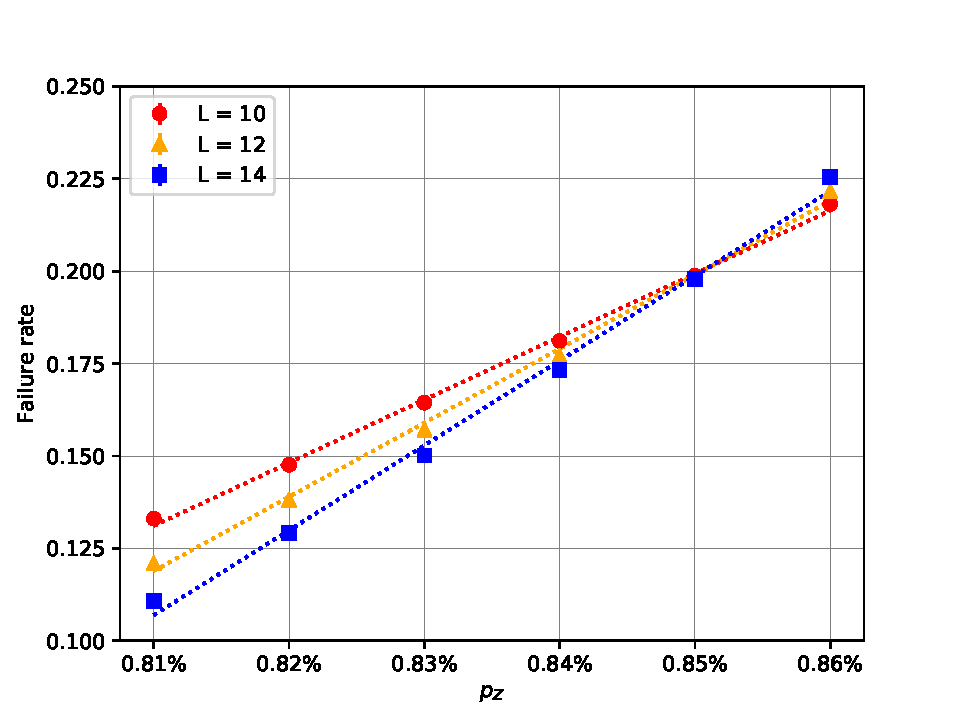
\includegraphics[width=.49\textwidth]{../graphs-paper2/fsf-dephasing-even.pdf}
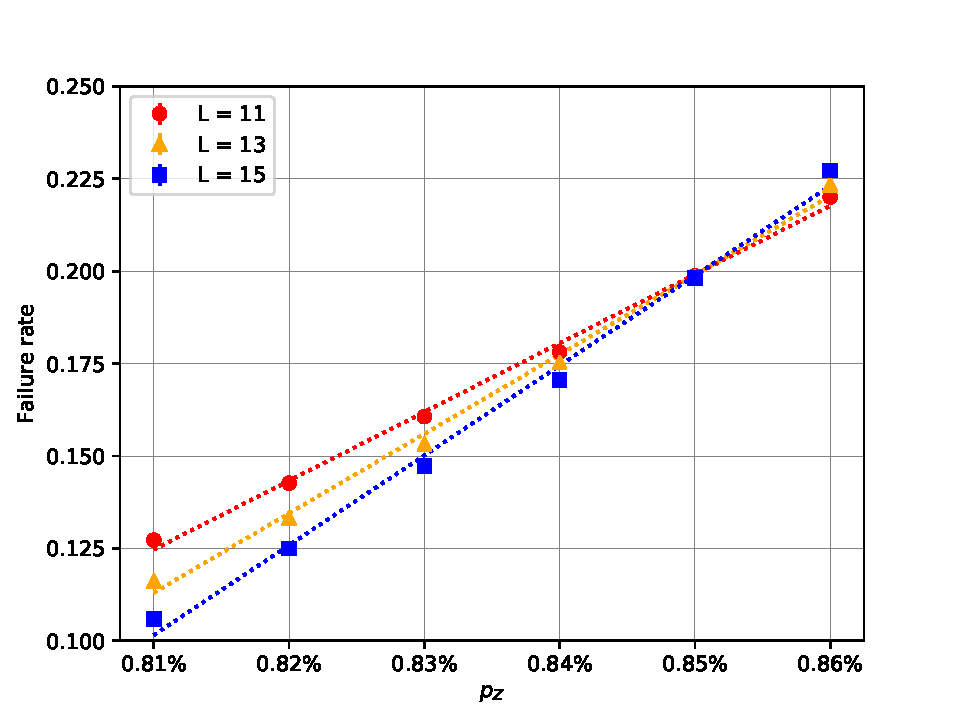
\includegraphics[width=.49\textwidth]{../graphs-paper2/fsf-dephasing-odd.pdf}

\noindent Fitting all points to a linear function $f(x) = A + Bx$, where $x=(p-p_{th})L^{\nu}$ for some $p_{th}$ and $\nu$: 
  
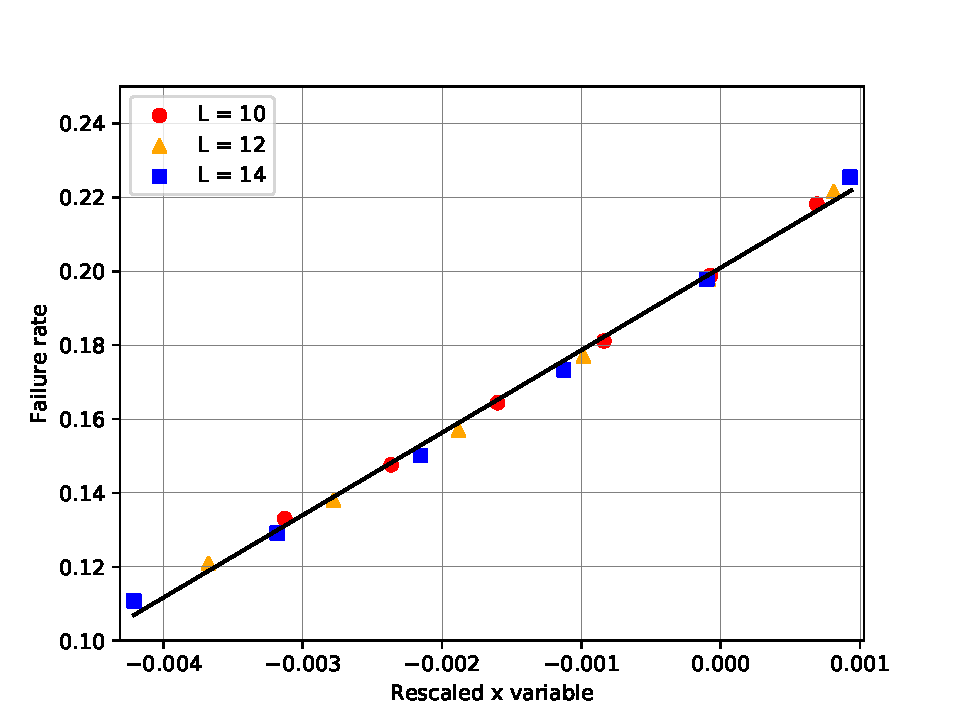
\includegraphics[width=.49\textwidth]{../graphs-paper2/fsf-dephasing-even-rescaled.pdf}
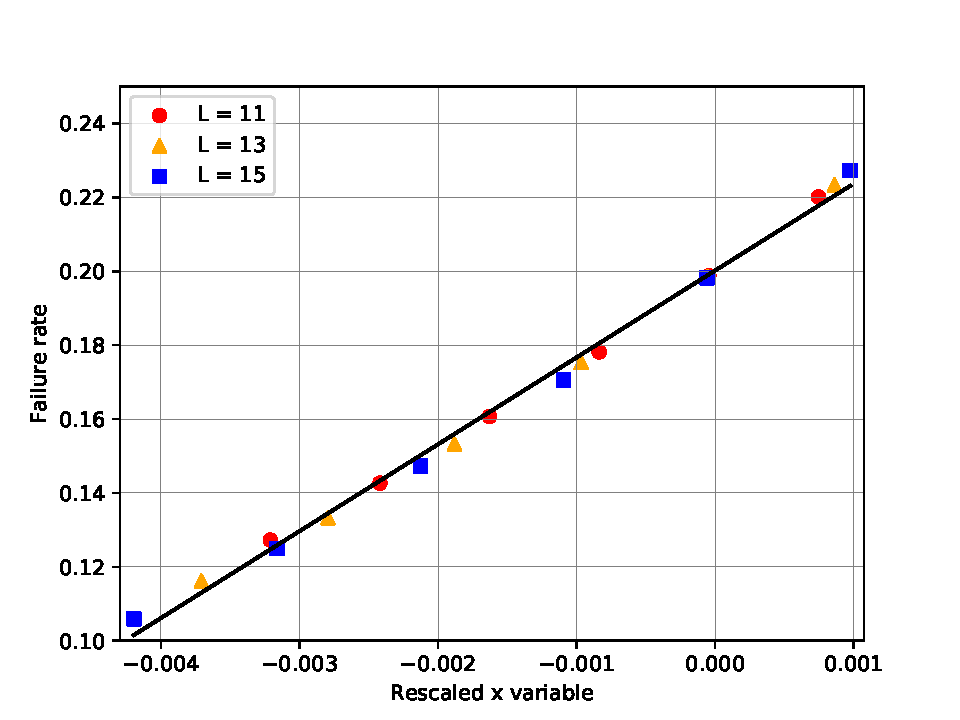
\includegraphics[width=.49\textwidth]{../graphs-paper2/fsf-dephasing-odd-rescaled.pdf}

\[  p_{even} = (0.851 \pm 0.006)\% \]
\[  p_{odd} = (0.851 \pm 0.008)\% \]
\clearpage 

Unified fit: \begin{center} 

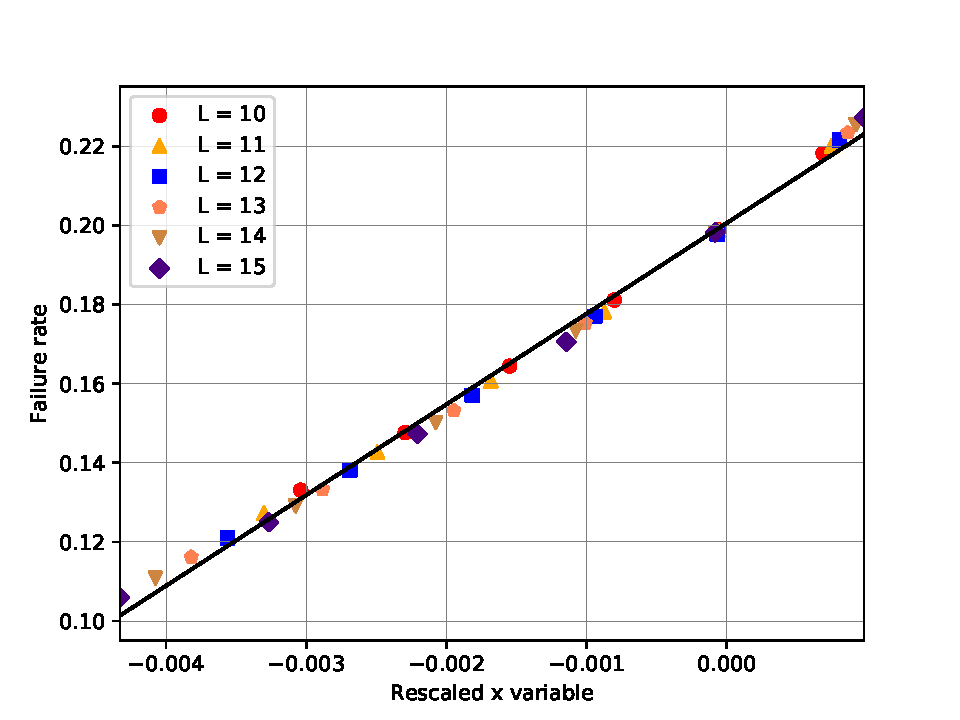
\includegraphics[width=.9\textwidth]{../graphs-paper2/fsf-dephasing-rescaled.pdf}
\[  p_{th} = (0.851 \pm 0.004)\% \] \end{center}
\clearpage 

\subsection*{ftw}
\noindent Increase of the failure rate with error probability: 
  
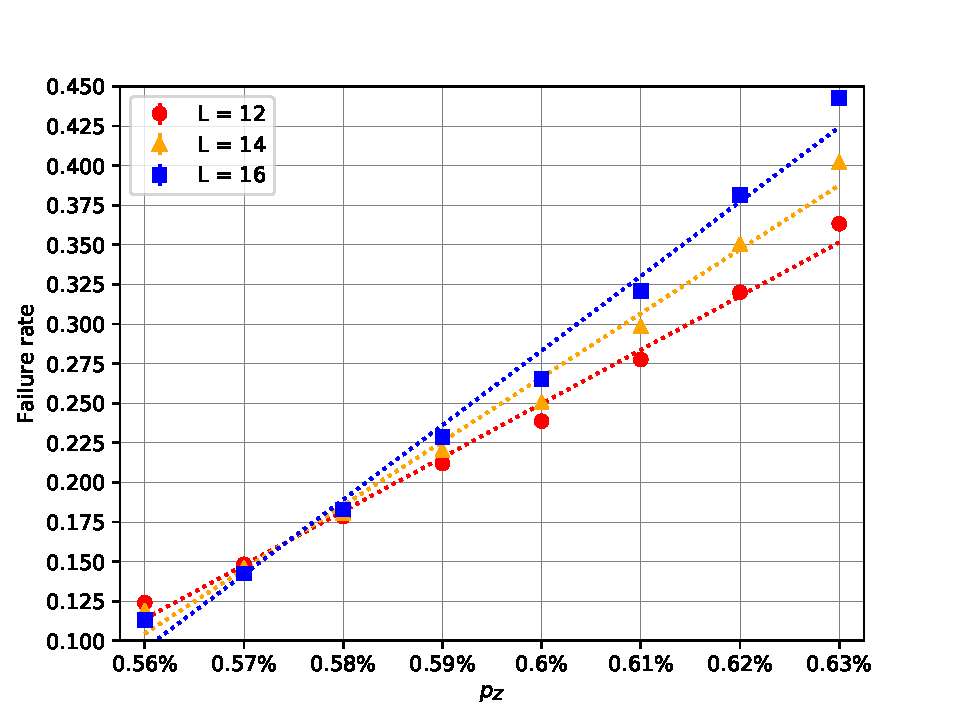
\includegraphics[width=.49\textwidth]{../graphs-paper2/ftw-dephasing-even.pdf}
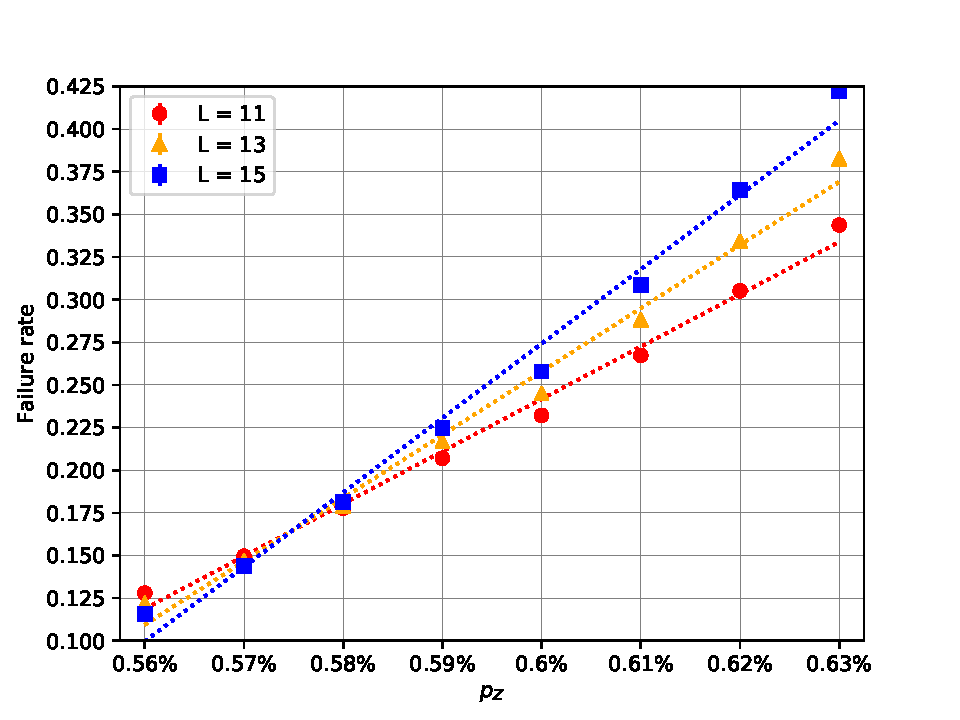
\includegraphics[width=.49\textwidth]{../graphs-paper2/ftw-dephasing-odd.pdf}

\noindent Fitting all points to a linear function $f(x) = A + Bx$, where $x=(p-p_{th})L^{\nu}$ for some $p_{th}$ and $\nu$: 
  
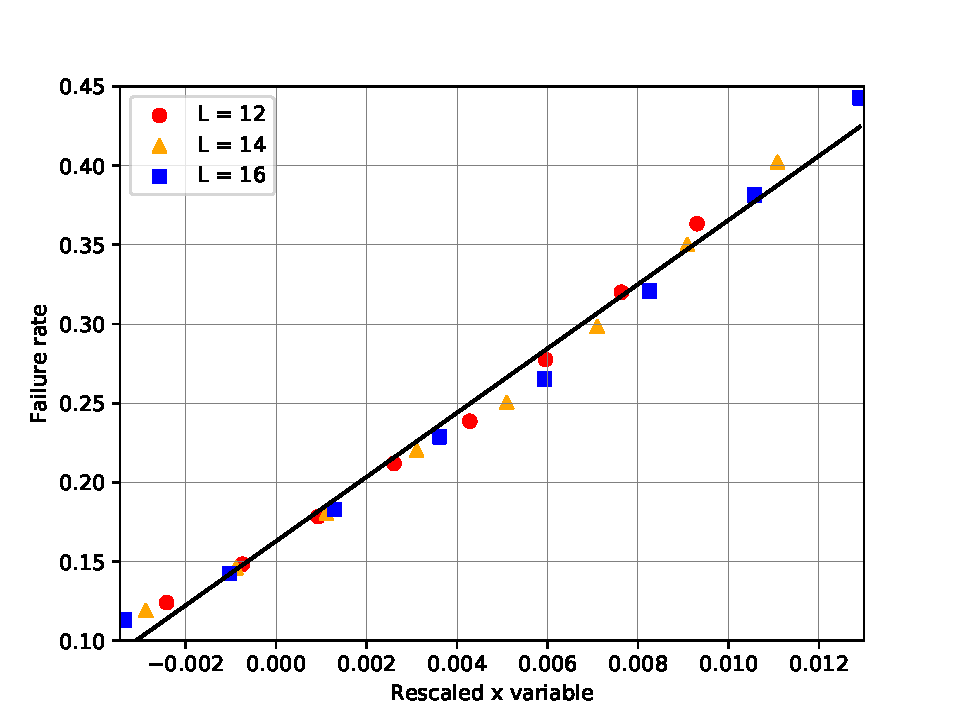
\includegraphics[width=.49\textwidth]{../graphs-paper2/ftw-dephasing-even-rescaled.pdf}
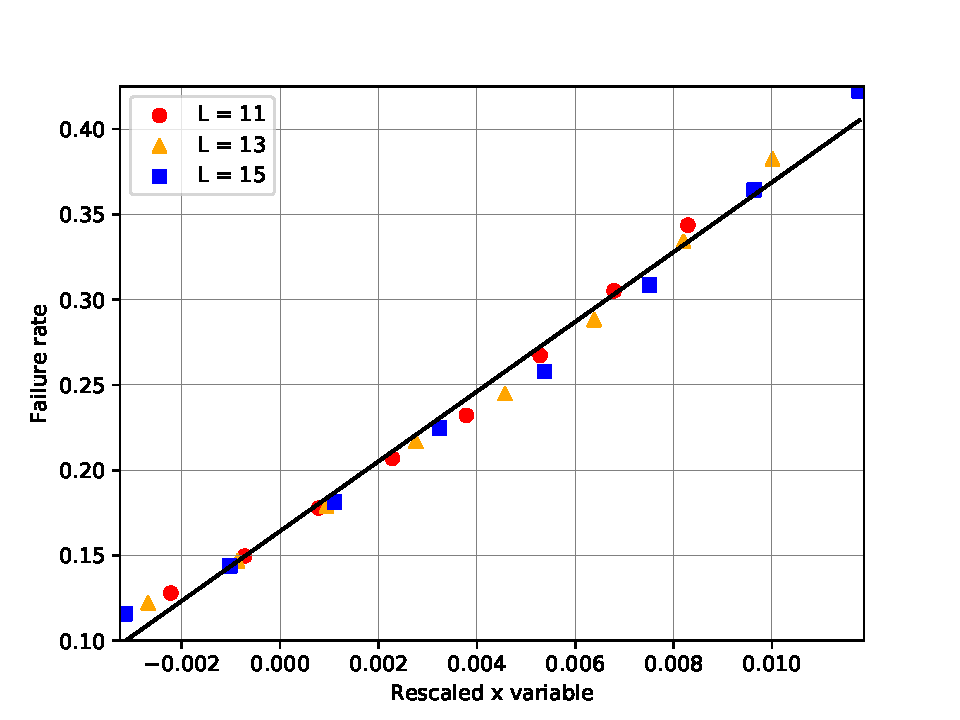
\includegraphics[width=.49\textwidth]{../graphs-paper2/ftw-dephasing-odd-rescaled.pdf}

\[  p_{even} = (0.574 \pm 0.011)\% \]
\[  p_{odd} = (0.575 \pm 0.01)\% \]
\clearpage 

Unified fit: \begin{center} 

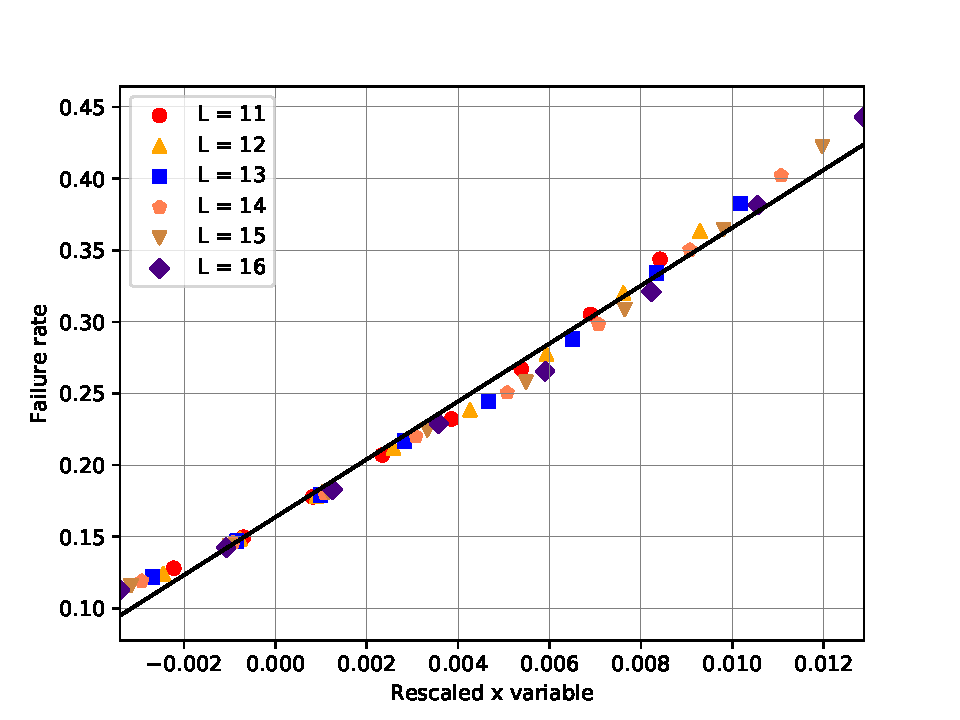
\includegraphics[width=.9\textwidth]{../graphs-paper2/ftw-dephasing-rescaled.pdf}
\[  p_{th} = (0.575 \pm 0.007)\% \] \end{center}
\clearpage 

\subsection*{hms}
\noindent Increase of the failure rate with error probability: 
  
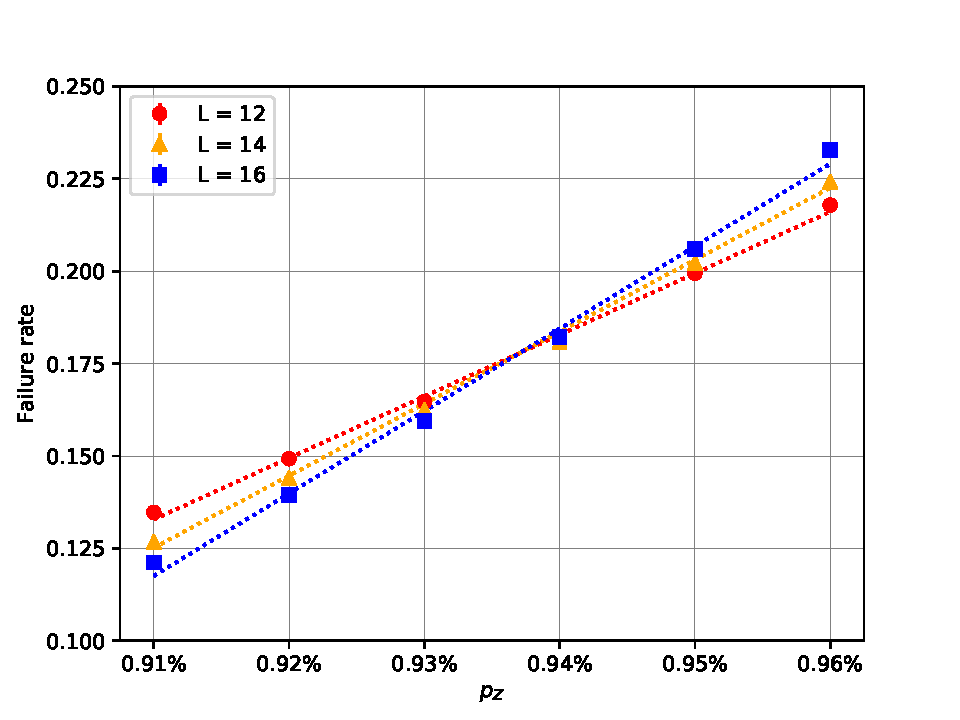
\includegraphics[width=.49\textwidth]{../graphs-paper2/hms-dephasing-even.pdf}
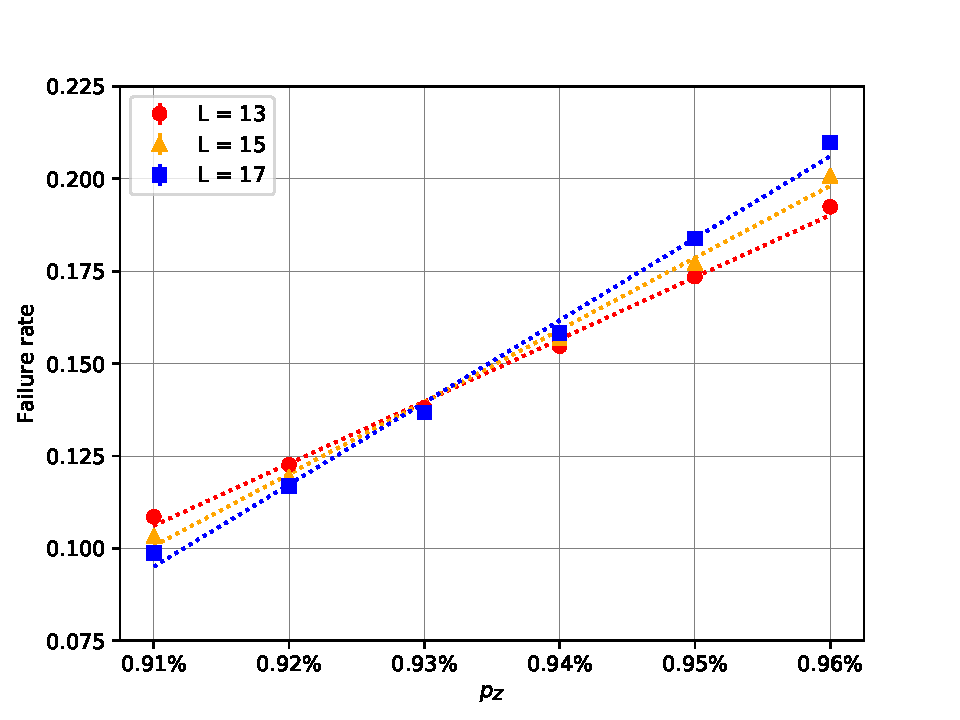
\includegraphics[width=.49\textwidth]{../graphs-paper2/hms-dephasing-odd.pdf}

\noindent Fitting all points to a linear function $f(x) = A + Bx$, where $x=(p-p_{th})L^{\nu}$ for some $p_{th}$ and $\nu$: 
  
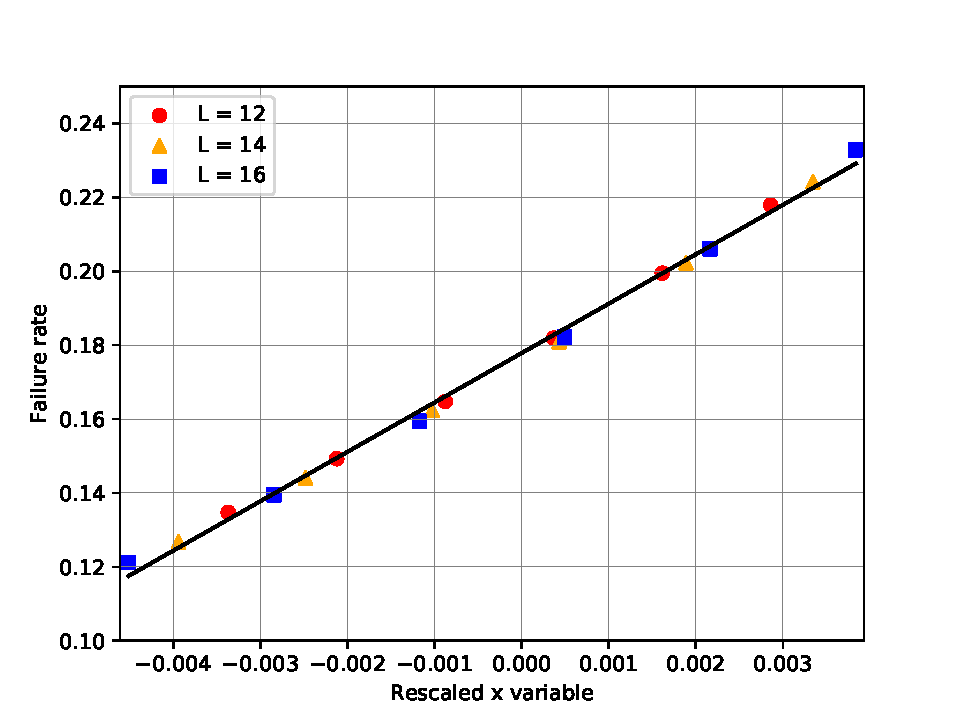
\includegraphics[width=.49\textwidth]{../graphs-paper2/hms-dephasing-even-rescaled.pdf}
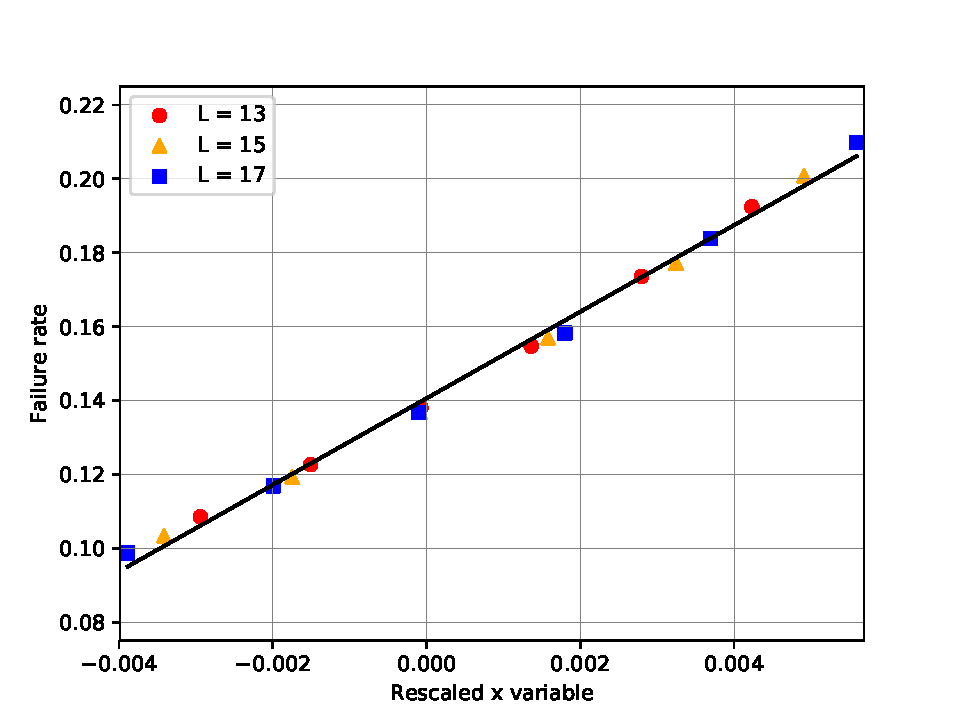
\includegraphics[width=.49\textwidth]{../graphs-paper2/hms-dephasing-odd-rescaled.pdf}

\[  p_{even} = (0.937 \pm 0.004)\% \]
\[  p_{odd} = (0.931 \pm 0.006)\% \]
\clearpage 

Unified fit: \begin{center} 

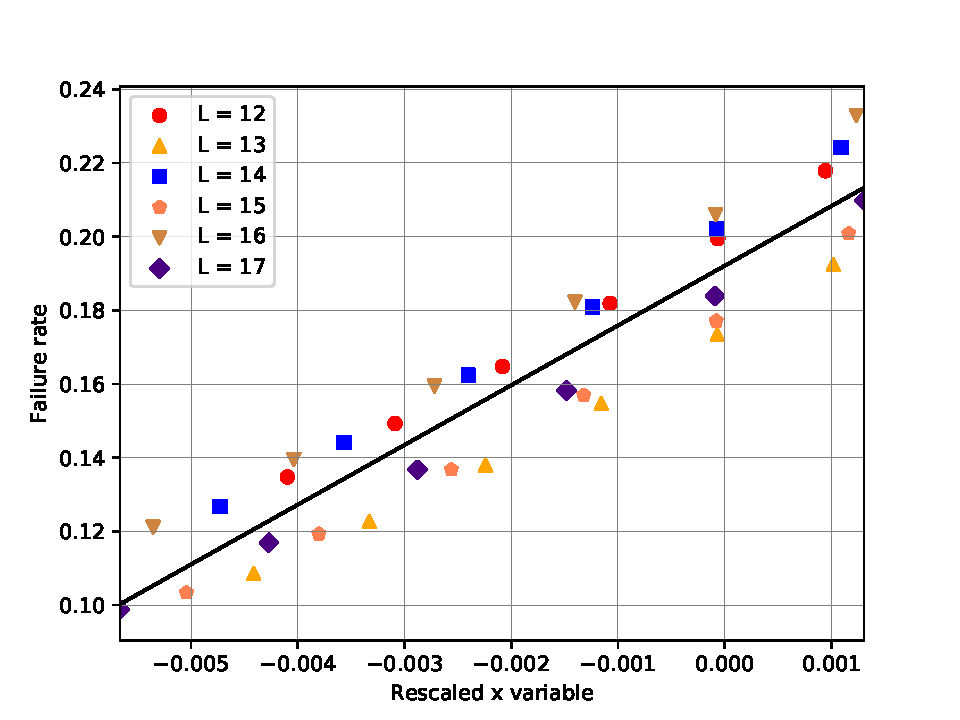
\includegraphics[width=.9\textwidth]{../graphs-paper2/hms-dephasing-rescaled.pdf}
\[  p_{th} = (0.951 \pm 0.027)\% \] \end{center}
\clearpage 

\subsection*{hst}
\noindent Increase of the failure rate with error probability: 
  
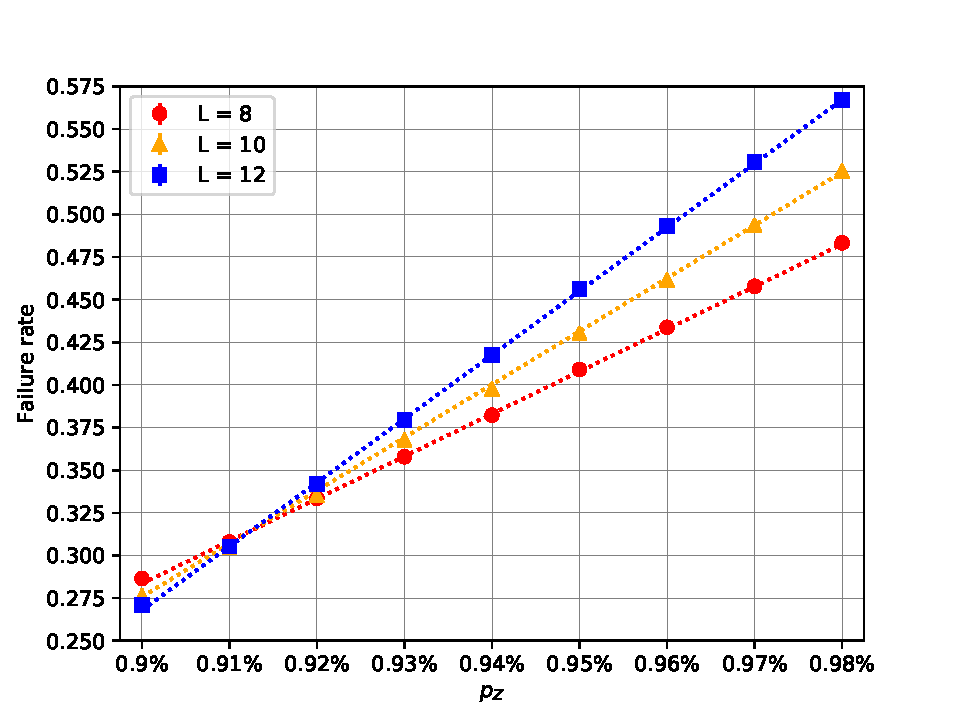
\includegraphics[width=.49\textwidth]{../graphs-paper2/hst-dephasing-even.pdf}
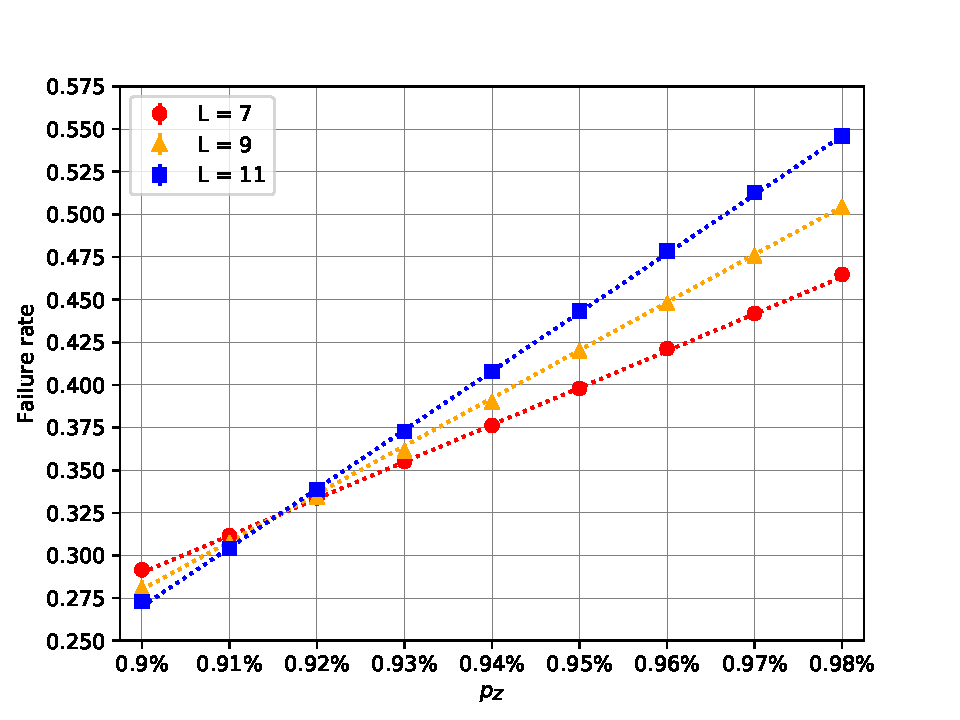
\includegraphics[width=.49\textwidth]{../graphs-paper2/hst-dephasing-odd.pdf}

\noindent Fitting all points to a linear function $f(x) = A + Bx$, where $x=(p-p_{th})L^{\nu}$ for some $p_{th}$ and $\nu$: 
  
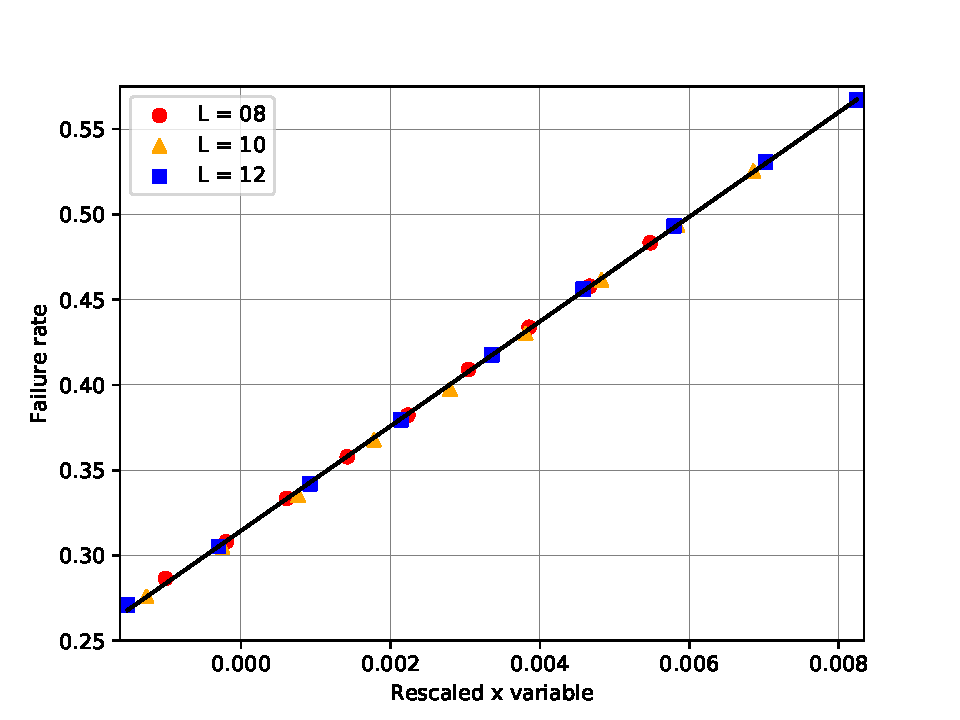
\includegraphics[width=.49\textwidth]{../graphs-paper2/hst-dephasing-even-rescaled.pdf}
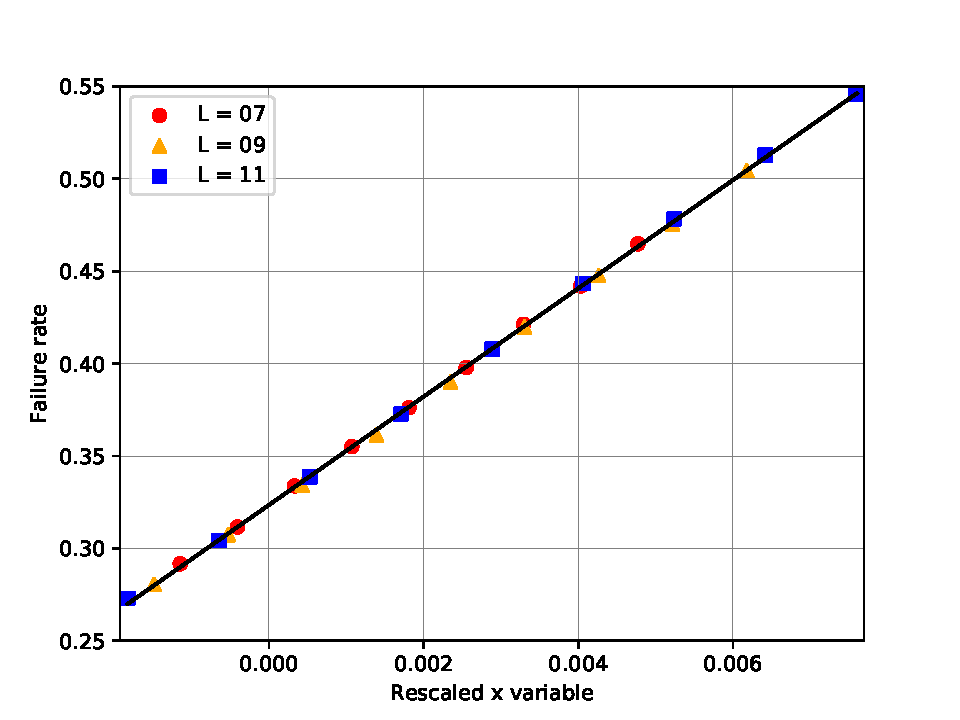
\includegraphics[width=.49\textwidth]{../graphs-paper2/hst-dephasing-odd-rescaled.pdf}

\[  p_{even} = (0.912 \pm 0.002)\% \]
\[  p_{odd} = (0.916 \pm 0.001)\% \]
\clearpage 

Unified fit: \begin{center} 

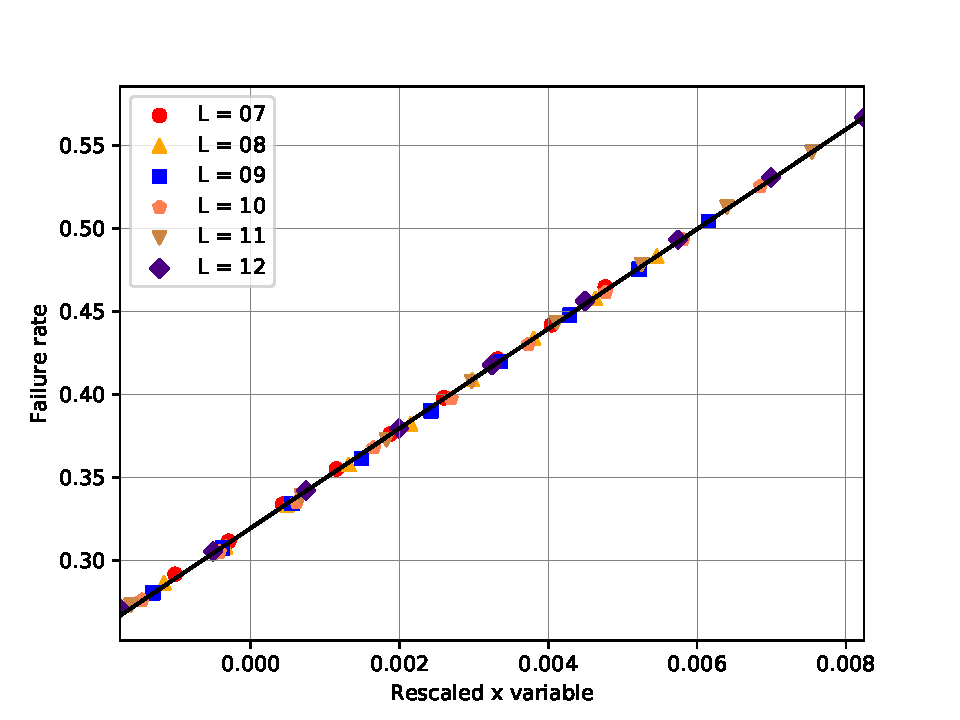
\includegraphics[width=.9\textwidth]{../graphs-paper2/hst-dephasing-rescaled.pdf}
\[  p_{th} = (0.914 \pm 0.001)\% \] \end{center}
\clearpage 

\subsection*{lcy}
\noindent Increase of the failure rate with error probability: 
  
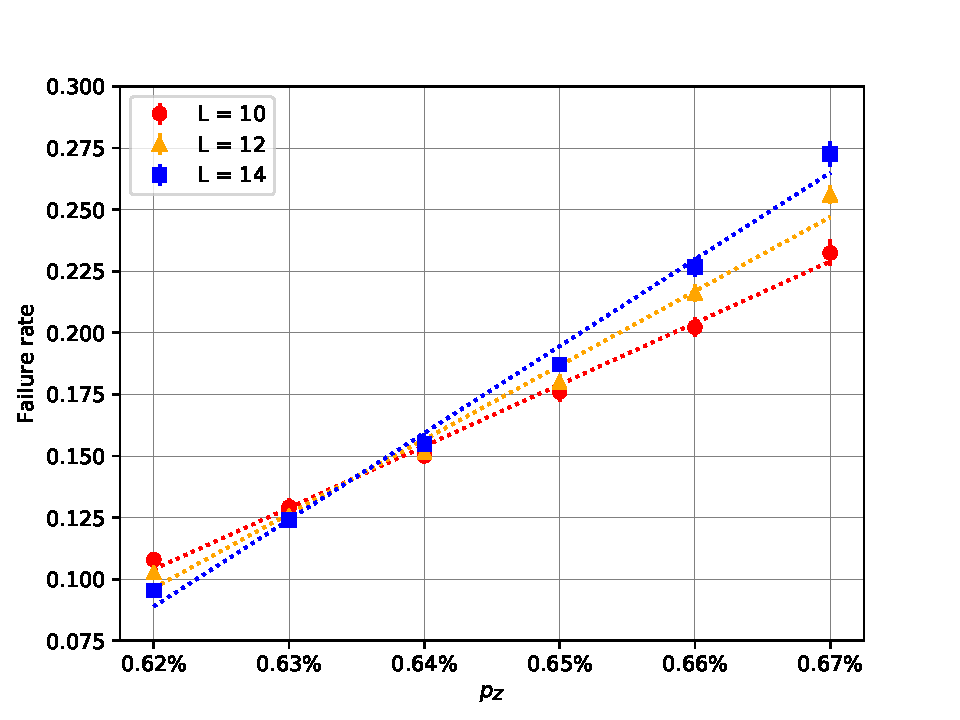
\includegraphics[width=.49\textwidth]{../graphs-paper2/lcy-dephasing-even.pdf}
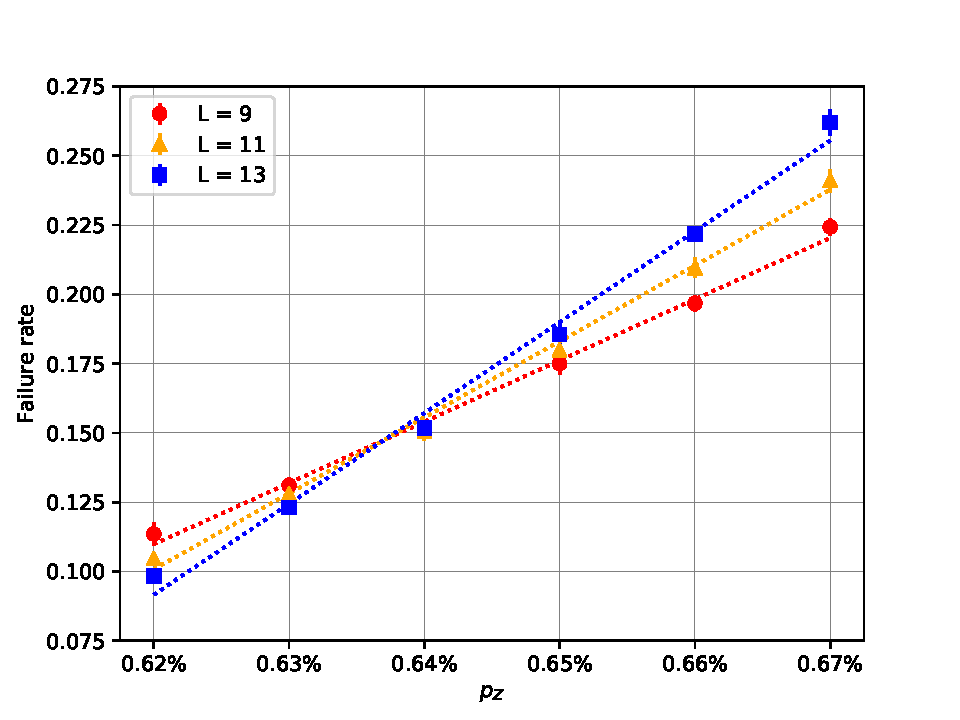
\includegraphics[width=.49\textwidth]{../graphs-paper2/lcy-dephasing-odd.pdf}

\noindent Fitting all points to a linear function $f(x) = A + Bx$, where $x=(p-p_{th})L^{\nu}$ for some $p_{th}$ and $\nu$: 
  
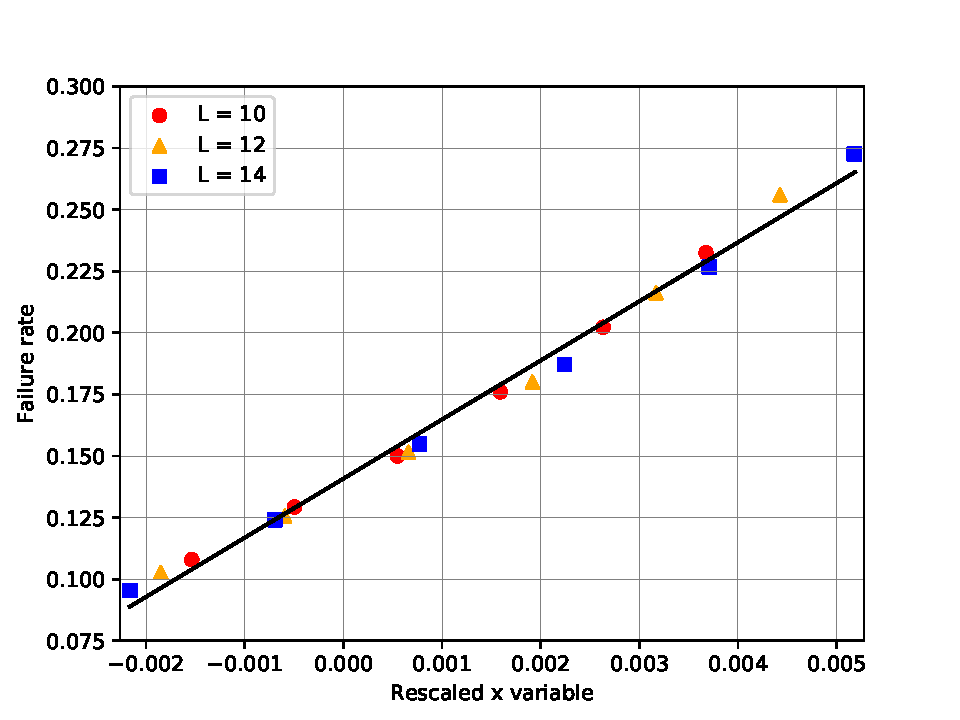
\includegraphics[width=.49\textwidth]{../graphs-paper2/lcy-dephasing-even-rescaled.pdf}
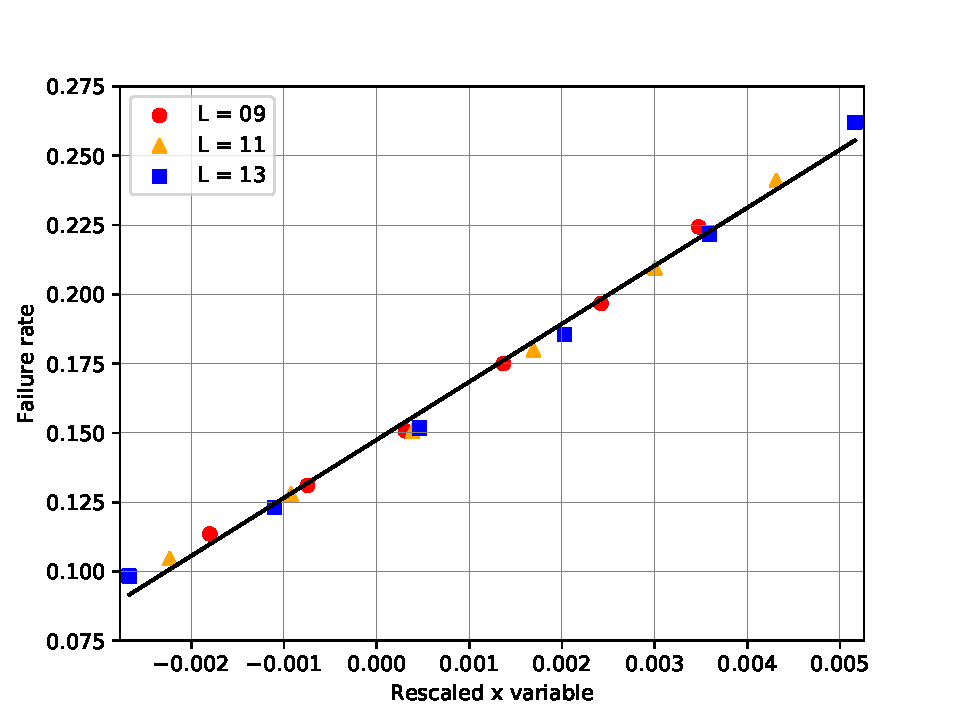
\includegraphics[width=.49\textwidth]{../graphs-paper2/lcy-dephasing-odd-rescaled.pdf}

\[  p_{even} = (0.635 \pm 0.007)\% \]
\[  p_{odd} = (0.637 \pm 0.005)\% \]
\clearpage 

Unified fit: \begin{center} 

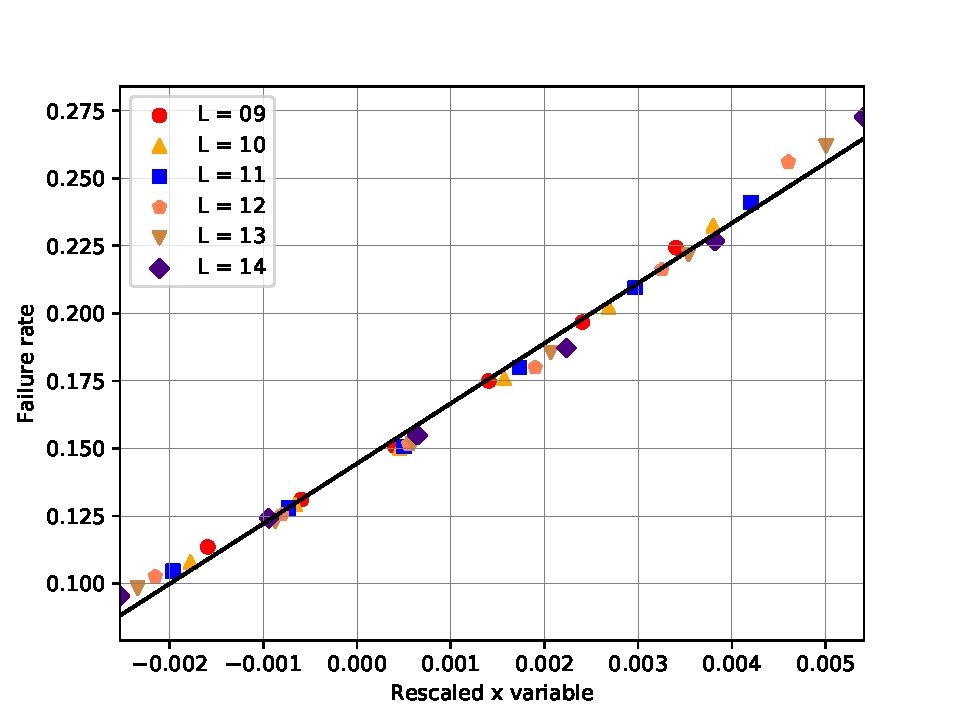
\includegraphics[width=.9\textwidth]{../graphs-paper2/lcy-dephasing-rescaled.pdf}
\[  p_{th} = (0.636 \pm 0.004)\% \] \end{center}
\clearpage 

\subsection*{mab}
\noindent Increase of the failure rate with error probability: 
  
\includegraphics[width=.49\textwidth]{../graphs-paper2/mab-dephasing-even.pdf}
\includegraphics[width=.49\textwidth]{../graphs-paper2/mab-dephasing-odd.pdf}

\noindent Fitting all points to a linear function $f(x) = A + Bx$, where $x=(p-p_{th})L^{\nu}$ for some $p_{th}$ and $\nu$: 
  
\includegraphics[width=.49\textwidth]{../graphs-paper2/mab-dephasing-even-rescaled.pdf}
\includegraphics[width=.49\textwidth]{../graphs-paper2/mab-dephasing-odd-rescaled.pdf}

\[  p_{even} = (0.476 \pm 0.014)\% \]
\[  p_{odd} = (0.474 \pm 0.014)\% \]
\clearpage 

Unified fit: \begin{center} 

\includegraphics[width=.9\textwidth]{../graphs-paper2/mab-dephasing-rescaled.pdf}
\[  p_{th} = (0.476 \pm 0.009)\% \] \end{center}
\clearpage 

\subsection*{mcf}
\noindent Increase of the failure rate with error probability: 
  
\includegraphics[width=.49\textwidth]{../graphs-paper2/mcf-dephasing-even.pdf}
\includegraphics[width=.49\textwidth]{../graphs-paper2/mcf-dephasing-odd.pdf}

\noindent Fitting all points to a linear function $f(x) = A + Bx$, where $x=(p-p_{th})L^{\nu}$ for some $p_{th}$ and $\nu$: 
  
\includegraphics[width=.49\textwidth]{../graphs-paper2/mcf-dephasing-even-rescaled.pdf}
\includegraphics[width=.49\textwidth]{../graphs-paper2/mcf-dephasing-odd-rescaled.pdf}

\[  p_{even} = (0.911 \pm 0.004)\% \]
\[  p_{odd} = (0.91 \pm 0.004)\% \]
\clearpage 

Unified fit: \begin{center} 

\includegraphics[width=.9\textwidth]{../graphs-paper2/mcf-dephasing-rescaled.pdf}
\[  p_{th} = (0.91 \pm 0.003)\% \] \end{center}
\clearpage 

\subsection*{mco}
\noindent Increase of the failure rate with error probability: 
  
\includegraphics[width=.49\textwidth]{../graphs-paper2/mco-dephasing-even.pdf}
\includegraphics[width=.49\textwidth]{../graphs-paper2/mco-dephasing-odd.pdf}

\noindent Fitting all points to a linear function $f(x) = A + Bx$, where $x=(p-p_{th})L^{\nu}$ for some $p_{th}$ and $\nu$: 
  
\includegraphics[width=.49\textwidth]{../graphs-paper2/mco-dephasing-even-rescaled.pdf}
\includegraphics[width=.49\textwidth]{../graphs-paper2/mco-dephasing-odd-rescaled.pdf}

\[  p_{even} = (1.096 \pm 0.003)\% \]
\[  p_{odd} = (1.098 \pm 0.003)\% \]
\clearpage 

Unified fit: \begin{center} 

\includegraphics[width=.9\textwidth]{../graphs-paper2/mco-dephasing-rescaled.pdf}
\[  p_{th} = (1.097 \pm 0.002)\% \] \end{center}
\clearpage 

\subsection*{mgc}
\noindent Increase of the failure rate with error probability: 
  
\includegraphics[width=.49\textwidth]{../graphs-paper2/mgc-dephasing-even.pdf}
\includegraphics[width=.49\textwidth]{../graphs-paper2/mgc-dephasing-odd.pdf}

\noindent Fitting all points to a linear function $f(x) = A + Bx$, where $x=(p-p_{th})L^{\nu}$ for some $p_{th}$ and $\nu$: 
  
\includegraphics[width=.49\textwidth]{../graphs-paper2/mgc-dephasing-even-rescaled.pdf}
\includegraphics[width=.49\textwidth]{../graphs-paper2/mgc-dephasing-odd-rescaled.pdf}

\[  p_{even} = (0.388 \pm 0.018)\% \]
\[  p_{odd} = (0.386 \pm 0.022)\% \]
\clearpage 

Unified fit: \begin{center} 

\includegraphics[width=.9\textwidth]{../graphs-paper2/mgc-dephasing-rescaled.pdf}
\[  p_{th} = (0.387 \pm 0.013)\% \] \end{center}
\clearpage 

\subsection*{pcu}
\noindent Increase of the failure rate with error probability: 
  
\includegraphics[width=.49\textwidth]{../graphs-paper2/pcu-dephasing-even.pdf}
\includegraphics[width=.49\textwidth]{../graphs-paper2/pcu-dephasing-odd.pdf}

\noindent Fitting all points to a linear function $f(x) = A + Bx$, where $x=(p-p_{th})L^{\nu}$ for some $p_{th}$ and $\nu$: 
  
\includegraphics[width=.49\textwidth]{../graphs-paper2/pcu-dephasing-even-rescaled.pdf}
\includegraphics[width=.49\textwidth]{../graphs-paper2/pcu-dephasing-odd-rescaled.pdf}

\[  p_{even} = (0.755 \pm 0.007)\% \]
\[  p_{odd} = (0.744 \pm 0.01)\% \]
\clearpage 

Unified fit: \begin{center} 

\includegraphics[width=.9\textwidth]{../graphs-paper2/pcu-dephasing-rescaled.pdf}
\[  p_{th} = (0.759 \pm 0.013)\% \] \end{center}
\clearpage 

\subsection*{pte}
\noindent Increase of the failure rate with error probability: 
  
\includegraphics[width=.49\textwidth]{../graphs-paper2/pte-dephasing-even.pdf}
\includegraphics[width=.49\textwidth]{../graphs-paper2/pte-dephasing-odd.pdf}

\noindent Fitting all points to a linear function $f(x) = A + Bx$, where $x=(p-p_{th})L^{\nu}$ for some $p_{th}$ and $\nu$: 
  
\includegraphics[width=.49\textwidth]{../graphs-paper2/pte-dephasing-even-rescaled.pdf}
\includegraphics[width=.49\textwidth]{../graphs-paper2/pte-dephasing-odd-rescaled.pdf}

\[  p_{even} = (0.876 \pm 0.008)\% \]
\[  p_{odd} = (0.877 \pm 0.006)\% \]
\clearpage 

Unified fit: \begin{center} 

\includegraphics[width=.9\textwidth]{../graphs-paper2/pte-dephasing-rescaled.pdf}
\[  p_{th} = (0.877 \pm 0.005)\% \] \end{center}
\clearpage 

\subsection*{pyr}
\noindent Increase of the failure rate with error probability: 
  
\includegraphics[width=.49\textwidth]{../graphs-paper2/pyr-dephasing-even.pdf}
\includegraphics[width=.49\textwidth]{../graphs-paper2/pyr-dephasing-odd.pdf}

\noindent Fitting all points to a linear function $f(x) = A + Bx$, where $x=(p-p_{th})L^{\nu}$ for some $p_{th}$ and $\nu$: 
  
\includegraphics[width=.49\textwidth]{../graphs-paper2/pyr-dephasing-even-rescaled.pdf}
\includegraphics[width=.49\textwidth]{../graphs-paper2/pyr-dephasing-odd-rescaled.pdf}

\[  p_{even} = (0.898 \pm 0.004)\% \]
\[  p_{odd} = (0.898 \pm 0.004)\% \]
\clearpage 

Unified fit: \begin{center} 

\includegraphics[width=.9\textwidth]{../graphs-paper2/pyr-dephasing-rescaled.pdf}
\[  p_{th} = (0.898 \pm 0.003)\% \] \end{center}
\clearpage 

\subsection*{qtz-x}
\noindent Increase of the failure rate with error probability: 
  
\includegraphics[width=.49\textwidth]{../graphs-paper2/qtz-x-dephasing-even.pdf}
\includegraphics[width=.49\textwidth]{../graphs-paper2/qtz-x-dephasing-odd.pdf}

\noindent Fitting all points to a linear function $f(x) = A + Bx$, where $x=(p-p_{th})L^{\nu}$ for some $p_{th}$ and $\nu$: 
  
\includegraphics[width=.49\textwidth]{../graphs-paper2/qtz-x-dephasing-even-rescaled.pdf}
\includegraphics[width=.49\textwidth]{../graphs-paper2/qtz-x-dephasing-odd-rescaled.pdf}

\[  p_{even} = (0.606 \pm 0.006)\% \]
\[  p_{odd} = (0.607 \pm 0.005)\% \]
\clearpage 

Unified fit: \begin{center} 

\includegraphics[width=.9\textwidth]{../graphs-paper2/qtz-x-dephasing-rescaled.pdf}
\[  p_{th} = (0.606 \pm 0.003)\% \] \end{center}
\clearpage 

\subsection*{rtw}
\noindent Increase of the failure rate with error probability: 
  
\includegraphics[width=.49\textwidth]{../graphs-paper2/rtw-dephasing-even.pdf}
\includegraphics[width=.49\textwidth]{../graphs-paper2/rtw-dephasing-odd.pdf}

\noindent Fitting all points to a linear function $f(x) = A + Bx$, where $x=(p-p_{th})L^{\nu}$ for some $p_{th}$ and $\nu$: 
  
\includegraphics[width=.49\textwidth]{../graphs-paper2/rtw-dephasing-even-rescaled.pdf}
\includegraphics[width=.49\textwidth]{../graphs-paper2/rtw-dephasing-odd-rescaled.pdf}

\[  p_{even} = (0.835 \pm 0.003)\% \]
\[  p_{odd} = (0.829 \pm 0.003)\% \]
\clearpage 

Unified fit: \begin{center} 

\includegraphics[width=.9\textwidth]{../graphs-paper2/rtw-dephasing-rescaled.pdf}
\[  p_{th} = (0.833 \pm 0.002)\% \] \end{center}
\clearpage 

\subsection*{sda}
\noindent Increase of the failure rate with error probability: 
  
\includegraphics[width=.49\textwidth]{../graphs-paper2/sda-dephasing-even.pdf}
\includegraphics[width=.49\textwidth]{../graphs-paper2/sda-dephasing-odd.pdf}

\noindent Fitting all points to a linear function $f(x) = A + Bx$, where $x=(p-p_{th})L^{\nu}$ for some $p_{th}$ and $\nu$: 
  
\includegraphics[width=.49\textwidth]{../graphs-paper2/sda-dephasing-even-rescaled.pdf}
\includegraphics[width=.49\textwidth]{../graphs-paper2/sda-dephasing-odd-rescaled.pdf}

\[  p_{even} = (0.729 \pm 0.004)\% \]
\[  p_{odd} = (0.728 \pm 0.004)\% \]
\clearpage 

Unified fit: \begin{center} 

\includegraphics[width=.9\textwidth]{../graphs-paper2/sda-dephasing-rescaled.pdf}
\[  p_{th} = (0.729 \pm 0.003)\% \] \end{center}
\clearpage 

\subsection*{smt}
\noindent Increase of the failure rate with error probability: 
  
\includegraphics[width=.49\textwidth]{../graphs-paper2/smt-dephasing-even.pdf}
\includegraphics[width=.49\textwidth]{../graphs-paper2/smt-dephasing-odd.pdf}

\noindent Fitting all points to a linear function $f(x) = A + Bx$, where $x=(p-p_{th})L^{\nu}$ for some $p_{th}$ and $\nu$: 
  
\includegraphics[width=.49\textwidth]{../graphs-paper2/smt-dephasing-even-rescaled.pdf}
\includegraphics[width=.49\textwidth]{../graphs-paper2/smt-dephasing-odd-rescaled.pdf}

\[  p_{even} = (0.729 \pm 0.016)\% \]
\[  p_{odd} = (0.73 \pm 0.014)\% \]
\clearpage 

Unified fit: \begin{center} 

\includegraphics[width=.9\textwidth]{../graphs-paper2/smt-dephasing-rescaled.pdf}
\[  p_{th} = (0.729 \pm 0.01)\% \] \end{center}
\clearpage 

\subsection*{swl}
\noindent Increase of the failure rate with error probability: 
  
\includegraphics[width=.49\textwidth]{../graphs-paper2/swl-dephasing-even.pdf}
\includegraphics[width=.49\textwidth]{../graphs-paper2/swl-dephasing-odd.pdf}

\noindent Fitting all points to a linear function $f(x) = A + Bx$, where $x=(p-p_{th})L^{\nu}$ for some $p_{th}$ and $\nu$: 
  
\includegraphics[width=.49\textwidth]{../graphs-paper2/swl-dephasing-even-rescaled.pdf}
\includegraphics[width=.49\textwidth]{../graphs-paper2/swl-dephasing-odd-rescaled.pdf}

\[  p_{even} = (0.652 \pm 0.003)\% \]
\[  p_{odd} = (0.655 \pm 0.002)\% \]
\clearpage 

Unified fit: \begin{center} 

\includegraphics[width=.9\textwidth]{../graphs-paper2/swl-dephasing-rescaled.pdf}
\[  p_{th} = (0.653 \pm 0.002)\% \] \end{center}
\clearpage 

\subsection*{sxd}
\noindent Increase of the failure rate with error probability: 
  
\includegraphics[width=.49\textwidth]{../graphs-paper2/sxd-dephasing-even.pdf}
\includegraphics[width=.49\textwidth]{../graphs-paper2/sxd-dephasing-odd.pdf}

\noindent Fitting all points to a linear function $f(x) = A + Bx$, where $x=(p-p_{th})L^{\nu}$ for some $p_{th}$ and $\nu$: 
  
\includegraphics[width=.49\textwidth]{../graphs-paper2/sxd-dephasing-even-rescaled.pdf}
\includegraphics[width=.49\textwidth]{../graphs-paper2/sxd-dephasing-odd-rescaled.pdf}

\[  p_{even} = (0.77 \pm 0.013)\% \]
\[  p_{odd} = (0.769 \pm 0.014)\% \]
\clearpage 

Unified fit: \begin{center} 

\includegraphics[width=.9\textwidth]{../graphs-paper2/sxd-dephasing-rescaled.pdf}
\[  p_{th} = (0.769 \pm 0.008)\% \] \end{center}
\clearpage 

\subsection*{tfa}
\noindent Increase of the failure rate with error probability: 
  
\includegraphics[width=.49\textwidth]{../graphs-paper2/tfa-dephasing-even.pdf}
\includegraphics[width=.49\textwidth]{../graphs-paper2/tfa-dephasing-odd.pdf}

\noindent Fitting all points to a linear function $f(x) = A + Bx$, where $x=(p-p_{th})L^{\nu}$ for some $p_{th}$ and $\nu$: 
  
\includegraphics[width=.49\textwidth]{../graphs-paper2/tfa-dephasing-even-rescaled.pdf}
\includegraphics[width=.49\textwidth]{../graphs-paper2/tfa-dephasing-odd-rescaled.pdf}

\[  p_{even} = (1.106 \pm 0.002)\% \]
\[  p_{odd} = (1.105 \pm 0.002)\% \]
\clearpage 

Unified fit: \begin{center} 

\includegraphics[width=.9\textwidth]{../graphs-paper2/tfa-dephasing-rescaled.pdf}
\[  p_{th} = (1.106 \pm 0.002)\% \] \end{center}
\clearpage 

\subsection*{ths}
\noindent Increase of the failure rate with error probability: 
  
\includegraphics[width=.49\textwidth]{../graphs-paper2/ths-dephasing-even.pdf}
\includegraphics[width=.49\textwidth]{../graphs-paper2/ths-dephasing-odd.pdf}

\noindent Fitting all points to a linear function $f(x) = A + Bx$, where $x=(p-p_{th})L^{\nu}$ for some $p_{th}$ and $\nu$: 
  
\includegraphics[width=.49\textwidth]{../graphs-paper2/ths-dephasing-even-rescaled.pdf}
\includegraphics[width=.49\textwidth]{../graphs-paper2/ths-dephasing-odd-rescaled.pdf}

\[  p_{even} = (1.076 \pm 0.004)\% \]
\[  p_{odd} = (1.078 \pm 0.004)\% \]
\clearpage 

Unified fit: \begin{center} 

\includegraphics[width=.9\textwidth]{../graphs-paper2/ths-dephasing-rescaled.pdf}
\[  p_{th} = (1.077 \pm 0.003)\% \] \end{center}
\clearpage 

\subsection*{tph}
\noindent Increase of the failure rate with error probability: 
  
\includegraphics[width=.49\textwidth]{../graphs-paper2/tph-dephasing-even.pdf}
\includegraphics[width=.49\textwidth]{../graphs-paper2/tph-dephasing-odd.pdf}

\noindent Fitting all points to a linear function $f(x) = A + Bx$, where $x=(p-p_{th})L^{\nu}$ for some $p_{th}$ and $\nu$: 
  
\includegraphics[width=.49\textwidth]{../graphs-paper2/tph-dephasing-even-rescaled.pdf}
\includegraphics[width=.49\textwidth]{../graphs-paper2/tph-dephasing-odd-rescaled.pdf}

\[  p_{even} = (0.572 \pm 0.009)\% \]
\[  p_{odd} = (0.575 \pm 0.004)\% \]
\clearpage 

Unified fit: \begin{center} 

\includegraphics[width=.9\textwidth]{../graphs-paper2/tph-dephasing-rescaled.pdf}
\[  p_{th} = (0.574 \pm 0.004)\% \] \end{center}
\clearpage 

\subsection*{ttv}
\noindent Increase of the failure rate with error probability: 
  
\includegraphics[width=.49\textwidth]{../graphs-paper2/ttv-dephasing-even.pdf}
\includegraphics[width=.49\textwidth]{../graphs-paper2/ttv-dephasing-odd.pdf}

\noindent Fitting all points to a linear function $f(x) = A + Bx$, where $x=(p-p_{th})L^{\nu}$ for some $p_{th}$ and $\nu$: 
  
\includegraphics[width=.49\textwidth]{../graphs-paper2/ttv-dephasing-even-rescaled.pdf}
\includegraphics[width=.49\textwidth]{../graphs-paper2/ttv-dephasing-odd-rescaled.pdf}

\[  p_{even} = (0.798 \pm 0.012)\% \]
\[  p_{odd} = (0.795 \pm 0.012)\% \]
\clearpage 

Unified fit: \begin{center} 

\includegraphics[width=.9\textwidth]{../graphs-paper2/ttv-dephasing-rescaled.pdf}
\[  p_{th} = (0.797 \pm 0.008)\% \] \end{center}
\clearpage 

\subsection*{unj}
\noindent Increase of the failure rate with error probability: 
  
\includegraphics[width=.49\textwidth]{../graphs-paper2/unj-dephasing-even.pdf}
\includegraphics[width=.49\textwidth]{../graphs-paper2/unj-dephasing-odd.pdf}

\noindent Fitting all points to a linear function $f(x) = A + Bx$, where $x=(p-p_{th})L^{\nu}$ for some $p_{th}$ and $\nu$: 
  
\includegraphics[width=.49\textwidth]{../graphs-paper2/unj-dephasing-even-rescaled.pdf}
\includegraphics[width=.49\textwidth]{../graphs-paper2/unj-dephasing-odd-rescaled.pdf}

\[  p_{even} = (0.989 \pm 0.005)\% \]
\[  p_{odd} = (0.989 \pm 0.005)\% \]
\clearpage 

Unified fit: \begin{center} 

\includegraphics[width=.9\textwidth]{../graphs-paper2/unj-dephasing-rescaled.pdf}
\[  p_{th} = (0.989 \pm 0.003)\% \] \end{center}
\clearpage 

\subsection*{vck}
\noindent Increase of the failure rate with error probability: 
  
\includegraphics[width=.49\textwidth]{../graphs-paper2/vck-dephasing-even.pdf}
\includegraphics[width=.49\textwidth]{../graphs-paper2/vck-dephasing-odd.pdf}

\noindent Fitting all points to a linear function $f(x) = A + Bx$, where $x=(p-p_{th})L^{\nu}$ for some $p_{th}$ and $\nu$: 
  
\includegraphics[width=.49\textwidth]{../graphs-paper2/vck-dephasing-even-rescaled.pdf}
\includegraphics[width=.49\textwidth]{../graphs-paper2/vck-dephasing-odd-rescaled.pdf}

\[  p_{even} = (0.653 \pm 0.003)\% \]
\[  p_{odd} = (0.653 \pm 0.003)\% \]
\clearpage 

Unified fit: \begin{center} 

\includegraphics[width=.9\textwidth]{../graphs-paper2/vck-dephasing-rescaled.pdf}
\[  p_{th} = (0.653 \pm 0.002)\% \] \end{center}
\clearpage 

\subsection*{vtx}
\noindent Increase of the failure rate with error probability: 
  
\includegraphics[width=.49\textwidth]{../graphs-paper2/vtx-dephasing-even.pdf}
\includegraphics[width=.49\textwidth]{../graphs-paper2/vtx-dephasing-odd.pdf}

\noindent Fitting all points to a linear function $f(x) = A + Bx$, where $x=(p-p_{th})L^{\nu}$ for some $p_{th}$ and $\nu$: 
  
\includegraphics[width=.49\textwidth]{../graphs-paper2/vtx-dephasing-even-rescaled.pdf}
\includegraphics[width=.49\textwidth]{../graphs-paper2/vtx-dephasing-odd-rescaled.pdf}

\[  p_{even} = (0.785 \pm 0.005)\% \]
\[  p_{odd} = (0.785 \pm 0.005)\% \]
\clearpage 

Unified fit: \begin{center} 

\includegraphics[width=.9\textwidth]{../graphs-paper2/vtx-dephasing-rescaled.pdf}
\[  p_{th} = (0.785 \pm 0.003)\% \] \end{center}
\clearpage 

\subsection*{wst}
\noindent Increase of the failure rate with error probability: 
  
\includegraphics[width=.49\textwidth]{../graphs-paper2/wst-dephasing-even.pdf}
\includegraphics[width=.49\textwidth]{../graphs-paper2/wst-dephasing-odd.pdf}

\noindent Fitting all points to a linear function $f(x) = A + Bx$, where $x=(p-p_{th})L^{\nu}$ for some $p_{th}$ and $\nu$: 
  
\includegraphics[width=.49\textwidth]{../graphs-paper2/wst-dephasing-even-rescaled.pdf}
\includegraphics[width=.49\textwidth]{../graphs-paper2/wst-dephasing-odd-rescaled.pdf}

\[  p_{even} = (0.295 \pm 0.015)\% \]
\[  p_{odd} = (0.296 \pm 0.013)\% \]
\clearpage 

Unified fit: \begin{center} 

\includegraphics[width=.9\textwidth]{../graphs-paper2/wst-dephasing-rescaled.pdf}
\[  p_{th} = (0.296 \pm 0.009)\% \] \end{center}
\clearpage
\section*{SPAM-seq}
\begin{center}
\noindent Dependence of the thresholds on the features of the graph: 
  
\includegraphics[width=.8\textwidth]{../graphs-paper2/thresholds-SPAM-seq-decoder.pdf}

\includegraphics[width=.8\textwidth]{../graphs-paper2/thresholds-SPAM-seq-cluster.pdf} \clearpage 

\clearpage
\subsection*{Ranking}
\begin{tabular}{|c|c|c|c|c|c|} \hline \bf Lattice & \bf Avg $d$ & \bf Avg $g$ & \bf Even Threshold & \bf Odd Threshold  & \bf Unified Threshold \\ \hline
\hline 
\color{blue}
wst &
\color{blue}
7.5 &
\color{blue}
3.0 &
\color{blue}
 $(0.607 \pm 0.006)\% $& 
\color{blue}
$(0.607 \pm 0.017)\% $ &
\color{blue}
$(0.607 \pm 0.005)\% $ \\
\hline \end{tabular}
\clearpage
\noindent Precision in terms of compute time: 
  
\includegraphics[width=.8\textwidth]{../graphs-paper2/time-SPAM-seq-0.pdf}

\end{center} 

\clearpage 

\subsection*{wst}
\noindent Increase of the failure rate with error probability: 
  
\includegraphics[width=.49\textwidth]{../graphs-paper2/wst-SPAM-seq-even.pdf}
\includegraphics[width=.49\textwidth]{../graphs-paper2/wst-SPAM-seq-odd.pdf}

\noindent Fitting all points to a linear function $f(x) = A + Bx$, where $x=(p-p_{th})L^{\nu}$ for some $p_{th}$ and $\nu$: 
  
\includegraphics[width=.49\textwidth]{../graphs-paper2/wst-SPAM-seq-even-rescaled.pdf}
\includegraphics[width=.49\textwidth]{../graphs-paper2/wst-SPAM-seq-odd-rescaled.pdf}

\[  p_{even} = (0.607 \pm 0.006)\% \]
\[  p_{odd} = (0.607 \pm 0.017)\% \]
\clearpage 

Unified fit: \begin{center} 

\includegraphics[width=.9\textwidth]{../graphs-paper2/wst-SPAM-seq-rescaled.pdf}
\[  p_{th} = (0.607 \pm 0.005)\% \] \end{center}
\clearpage
\end{document}
